\documentclass[11pt,a4paper]{article}
\usepackage[T1]{fontenc}
\usepackage[utf8]{inputenc}
\usepackage{lmodern,microtype}
\usepackage[margin=25mm]{geometry}
\usepackage{amsmath,amssymb,amsthm,mathtools,bm}
\usepackage{booktabs,tabularx,array,longtable,float}
\usepackage{enumitem}
\usepackage{xcolor,tikz}
\usetikzlibrary{arrows.meta,positioning,shapes.geometric}
\usepackage[colorlinks=true,linkcolor=blue!45!black,citecolor=blue!45!black,urlcolor=blue!45!black]{hyperref}
\usepackage{bookmark}
\hypersetup{pdftitle={DYSANOS II: Smooth SANOS-Type Equity Option Market Models},pdfsubject={Martingale product lifts, stochastic smoothing, DLV drift, Bates representation and consistent recalibration},pdfauthor={},pdfkeywords={SANOS, DYSANOS, martingale, discrete local volatility, stochastic volatility, recalibration}}
\setcounter{tocdepth}{1}
\usepackage{fancyhdr}
\pagestyle{fancy}\fancyhf{}
\fancyhead[L]{\small DYSANOS II: smooth martingale market models}
\fancyhead[R]{\small Research manuscript}
\fancyfoot[C]{\thepage}
\setlength{\headheight}{14pt}
\setlength{\emergencystretch}{2em}
\setlist{nosep,topsep=5pt}
\numberwithin{equation}{section}
\newtheorem{theorem}{Theorem}[section]
\newtheorem{proposition}[theorem]{Proposition}
\newtheorem{lemma}[theorem]{Lemma}
\newtheorem{corollary}[theorem]{Corollary}
\theoremstyle{definition}\newtheorem{definition}[theorem]{Definition}
\newtheorem{assumption}[theorem]{Assumption}
\theoremstyle{remark}\newtheorem{remark}[theorem]{Remark}
\newcommand{\Q}{\mathbb Q}\newcommand{\Pp}{\mathbb P}
\newcommand{\E}{\mathbb E}\newcommand{\R}{\mathbb R}
\newcommand{\F}{\mathcal F}\newcommand{\G}{\mathcal G}
\newcommand{\dd}{\,\mathrm d}\newcommand{\dt}{\,\mathrm dt}
\newcommand{\ind}{\mathbf 1}\newcommand{\diag}{\operatorname{diag}}
\newcommand{\Ran}{\operatorname{Ran}}\newcommand{\rank}{\operatorname{rank}}
\newcommand{\KL}{\operatorname{KL}}\newcommand{\ess}{\operatorname{ESS}}
\newcommand{\Black}{\mathcal B}\newcommand{\LC}{\mathcal L}
\newcommand{\bq}{\boldsymbol q}\newcommand{\cx}{\preceq_{\mathrm{cx}}}
\title{\textbf{DYSANOS II}\\[3mm]
Smooth SANOS-Type Equity Option Market Models\\
with Static and Dynamic No-Arbitrage Guarantees\\[3mm]
\large Density-coordinate drift restrictions, Black product lifts,\\
front settlement and consistent recalibration}
\author{}
\date{25 September 2026}
\begin{document}
\maketitle
\begin{abstract}
A useful equity option market simulator must reprice the same surviving contracts as the market evolves, generate realistic statistical scenarios, and avoid both cross-sectional and dynamic arbitrage. We develop a constructive route from a finite discrete-local-volatility (DLV) market to smooth SANOS-type option dynamics. First, we show that the Wiese density-coordinate drift restriction is the exact non-front-maturity reformulation of Wissel's finite-option drift restriction. Second, we identify the two boundary questions that this identity does not settle: terminal consistency at the front expiry and prices between quoted strikes. We construct a bounded latent martingale $X$ and an independent Black martingale $Y$, and price calls on $S=XY$ by conditional expectation. At model expiries this gives finite Black mixtures, smooth in strike, with true-martingale prices and exact settlement. An explicit finite-state construction supplies a finite-mixture surface for every maturity; a Brownian revelation construction supplies continuous spot paths at prescribed model expiries. The independent-product and general-background principles are inherited from SANOS. Their conditional formulation here includes explicit stochastic-volatility drift calculations and a concrete model with stochastic volatility of volatility. The Black kernel is then replaced by its full conditional pricing kernel. The induced smooth drift restriction has the Carmona--Nadtochiy covariance form, with a predictable jump correction when required.

Exact agreement with protected DLV quotes is obtained by joint calibration, not by adding positive smoothing to unchanged atomic weights. We prove local feasibility for strictly admissible finite books and distinguish initial quote matching from preservation of a preassigned entire grid process. Finally, we formulate a CRC-inspired historical calibration programme: construct admissible $Q$-dynamics first, estimate physical dynamics only through permitted risk premia, and preserve surviving prices at parameter resets. Structural identities, numerical discretisation and sample-based OCE diagnostics are treated separately. A dedicated Bates analysis proves the finite-Black-mixture representation obstruction, derives an exact continuous mixing representation, and distinguishes these oracle-specific facts from the existence of finite SANOS dynamics. It also supplies exact projection diagnostics, terminal rigidity results and alternative dynamic completions of directly calibrated marginals.
\end{abstract}
\vspace{2mm}
\noindent\textbf{Keywords.} Option market simulation; SANOS; discrete local volatility; martingale measures; smooth option surfaces; consistent recalibration; deep hedging.
\newpage\tableofcontents
\newpage

\section{Introduction}
\label{sec:intro}
\subsection{From equity option simulation to smooth dynamic surfaces}
Deep hedging learns trading rules from repeated market scenarios rather than from a prescribed analytic hedge. If options are themselves hedging instruments, the training environment must generate their joint evolution with spot, including the returns of each \emph{fixed cash-strike, fixed calendar-expiry} contract held by the strategy. Historical observations alone give relatively few independent episodes, particularly in stressed regimes. A market simulator therefore becomes part of the economic specification of the learning problem: defects in simulated prices can be learned as artificial trading opportunities.

Wiese, Bai, Wood and Buehler's \emph{Deep Hedging: Learning to Simulate Equity Option Markets} \cite{Wiese2019} established an important link between data-driven scenario generation and the DLV representation. Positivity in DLV coordinates protects the discrete cross-section against static arbitrage. The learned statistical transition is a separate object, however; a statically admissible decoder alone does not construct one equivalent measure under which every surviving option is a martingale. This distinction is particularly important when the quoted lattice rolls with spot and time.

There is also an interpolation problem. For $K=(1-\theta)K_i+\theta K_{i+1}$, convexity requires
\begin{equation}
 C(T,K)\leq (1-\theta)C(T,K_i)+\theta C(T,K_{i+1}),\qquad 0\leq\theta\leq1.
 \label{eq:chord}
\end{equation}
Thus the linear chord is the \emph{most expensive} convex interpolation between its endpoints. Here ``expensive'' means a high option price, not high computational complexity. Linear interpolation is cheap to compute. Its economic drawback is the upper-envelope price between quotes and the concentration of the implied distribution at grid knots; it does not produce a smooth density. A hedging agent trained on this envelope may face systematically distorted off-grid trading costs. This concern connects to Buehler's \emph{Expensive martingales} \cite{Expensive}.

SANOS \cite{SANOS} replaces this envelope by positive mixtures of smooth pricing kernels, with a particularly transparent Black implementation. Its combination of smoothness, inexpensive evaluation and constrained calibration makes it a natural decoder for an equity option market simulator. At a common set of fitted quotes a convex smooth fit lies below the corresponding linear chords, and can therefore supply less expensive off-grid prices. This is a comparison after calibration; smoothing a \emph{fixed} atomic distribution instead increases convex-payoff values. These two statements concern different operations.

Buehler, Horv\'ath and Kratsios's DYSANOS \cite{DYSANOS}, referred to here as \emph{DYSANOS I}, takes the first generative step using smooth SANOS surfaces. It combines a static arbitrage-free representation with estimated statistical state dynamics and investigates dynamic arbitrage empirically. The later supplied statistical draft, Version~2.0 with Wiese as a coauthor \cite{DYSANOSv2}, substantially develops the fitted simulator while expressly limiting its guarantee to static arbitrage. The present paper uses \emph{DYSANOS II} as a working label for a conditional-law research extension, distinct from that version number: common risk-neutral dynamics and settlement are part of the constructed model, but are not thereby proved for the existing fitted simulator. Historical realism remains an estimation objective, not a consequence of the no-arbitrage theorem.

\subsection{Related literature and the precise gap}
The market-model approach specifies dynamics of traded options alongside spot. Wissel's 2007 finite-option paper \cite{Wissel2007}, and the corresponding work collected in his thesis \cite{WisselThesis}, are the relevant discrete predecessors. They should be distinguished from Schweizer--Wissel's continuous-strike, single-maturity model \cite{SWMulti} and their fixed-strike term-structure model \cite{SWTerm}. Section~\ref{sec:finite} identifies an exact change of coordinates for the non-front finite-grid drift restriction. It does not identify all front conventions or all admissible coefficient classes across these papers.

Carmona--Nadtochiy \cite{CN2009,CN2008} develop a local-volatility codebook with a drift restriction and a spot-consistency boundary. Their subsequent tangent L\'evy models \cite{CN2012}, and the option HJM formulation of Kallsen--Kr\"uhner \cite{KK2015}, treat jump codebooks. They make clear why positive cross-sectional parameters are insufficient: the evolving codebook must remain a conditional description of the same market. The density-product identity derived below is the finite-grid and continuous-strike expression of this compatibility.

Gambara--Teichmann's consistent recalibration models \cite{CRC} permit parameters of a tractable risk-neutral model to change while a Hull--White-type extension compensates so that the evolved option surface is retained. Their generalised Bates example supplies inspiration for our \emph{order of operations}: evolve, propose a parameter update, then solve a price-preserving correction. Our correction acts on conditional distributions and SANOS coordinates. It is not obtained by substituting SANOS parameters into their theorem without checking admissibility.

Cont--da Fonseca \cite{ContFonseca} and Cont--Fonseca--Durrleman \cite{CFD} establish an empirical factor perspective on implied-volatility dynamics. Cont--Vuleti\'c \cite{ContVuletic} and VolGAN \cite{VolGAN} pursue realistic scenario generation with cross-sectional arbitrage control. Their contribution should not be described as ignoring arbitrage or surface dynamics. The distinction relevant here is that cross-sectional control and statistical fidelity do not, on their own, furnish the conditional pricing tower and terminal settlement proved below.

Cohen--Reisinger--Wang \cite{CRW} derive an HJM-type drift restriction and give hard constraints preserving a statically admissible factor domain. Their finite-factor implementation also constructs factors to reduce violations of the dynamic restriction, while Remark~2 explicitly distinguishes a rolling liquid lattice from fixed contracts. It would therefore be inaccurate to call their theory merely a penalty method. The comparison here is with a construction whose common conditional-expectation law makes the full stated family of prices martingales, rather than with a numerical objective that only reduces a drift residual.

Further foundations are Dupire's pricing identity \cite{Dupire}, the DLV construction of Buehler--Ryskin \cite{DLV}, Andreasen--Huge's interpolation scheme \cite{AH}, and martingale coupling in convex order \cite{Strassen,Kellerer}. Deep hedging \cite{DeepHedging} motivates the joint simulation objective. Utility-based drift removal \cite{OCE} provides a complementary diagnostic and measure-selection tool, but cannot create an equivalent martingale measure when the required span or support conditions fail.

\subsection{Contributions, scope and organisation}
The first result is the Wiese--Wissel drift equivalence in Section~\ref{sec:finite}. Section~\ref{sec:gaps} explains why a finite-grid drift identity leaves both the front boundary and a nonlinear interpolation open. Section~\ref{sec:product} gives the smooth product theorem and an explicit all-maturity example. Section~\ref{sec:stochY} extends the smoothing factor to time-varying and stochastic volatility, with a complete generator proof. Section~\ref{sec:matching} proves a local exact-fit result and specifies what common-node agreement means. Section~\ref{sec:continuous} derives the continuous covariance drift and its relation to Carmona--Nadtochiy. Section~\ref{sec:bates} adds the Bates representation and nonrepresentation results, exact residual diagnostics, terminal rigidity theorems and direct-calibration alternatives. Sections~\ref{sec:front}--\ref{sec:crc} complete the front, regridding, physical-measure and recalibration programme. Section~\ref{sec:statistical-bridge} reconciles the construction with the supplied statistical DYSANOS Version~2.0, including its two term structures and the distinction between inherited ideas and additional results. Section~\ref{sec:testing} states what numerical tests can and cannot certify.

The scope is deliberately precise. We prove absence of arbitrage for every finite portfolio of the constructed spot and option family under the usual admissibility restriction on trading strategies. We do not assert a large-market theorem for arbitrary infinite portfolios. We do not prove that every learned DLV volatility field has a global solution, that every historical surface can be represented with a fixed number of Black components, or that a finite numerical sweep establishes a universal existence claim. No new empirical performance results are asserted. Section~\ref{sec:bates} reports findings from the supplied Bates analyses with their provenance and unresolved audit limitations explicitly stated.

\section{A reminder of the finite-grid Wiese--Wissel drift condition}
\label{sec:finite}
\subsection{Contracts, butterflies and the discrete Dupire identity}
We work at zero interest and dividend rates on a finite horizon. Equivalently, an appropriate deterministic carry normalisation may first be applied. All martingale statements refer to a common measure $\Q$ and the market filtration. Fix cash strikes
\[
 0<K_0<K_1<\cdots<K_{N+1}
\]
and calendar expiries $T_1<\cdots<T_M$. On a trading slab $[T_{r-1},T_r)$ write $C_n^m(t)=C_t(T_m,K_n)$. A non-front maturity has $m>r$, so both $T_{m-1}$ and $T_m$ are live. Put $d_n=K_{n+1}-K_n$ and define interior butterflies
\begin{equation}
 q_n^m=\frac{C_{n+1}^m-C_n^m}{d_n}
       -\frac{C_n^m-C_{n-1}^m}{d_{n-1}},\qquad n=1,\ldots,N.
 \label{eq:butterfly}
\end{equation}
The $q_n^m$ are dimensionless slope differences. If the conditional law is supported on the entire finite grid, augment them by
\[
 q_0^m=1+\frac{C_1^m-C_0^m}{d_0},\qquad
 q_{N+1}^m=-\frac{C_{N+1}^m-C_N^m}{d_N},
\]
with $C_0^m=S_t-K_0$, $C_{N+1}^m=0$. Then
\begin{equation}
 \sum_iq_i^m=1,\quad \sum_iK_iq_i^m=S_t,\quad
 C_n^m=\sum_iq_i^m(K_i-K_n)^+.
 \label{eq:finite-density}
\end{equation}
When the true law has tails beyond the grid, \eqref{eq:butterfly} still defines valid interior butterflies, but the artificial boundary calls in \eqref{eq:finite-density} must not be substituted for the true tail prices.

For $q_n^m>0$ define the backward discrete local variance
\begin{equation}
 \ell_n^m=\frac{C_n^m-C_n^{m-1}}{\omega_n^m q_n^m},
 \qquad
 \omega_n^m=\frac{K_n^2(T_m-T_{m-1})}{K_{n+1}-K_{n-1}}.
 \label{eq:dupire-discrete}
\end{equation}
This is an \emph{exact coordinate identity} on a finite book. It is not an assertion that a finite difference equals a continuum derivative. Positivity of its numerator and denominator places the coordinates in the interior static-arbitrage domain. Degenerate zero-spread or zero-butterfly states require a boundary representation rather than division by zero.

\subsection{The covariance drift and its converse}
Let all live calls and spot be continuous local martingales, and write
\begin{equation}
 dC_n^m=\Lambda_n^m\cdot dW^Q,\quad dq_n^m=\psi_n^m\cdot dW^Q,\quad
 d\ell_n^m=\alpha_n^m\dt+\beta_n^m\cdot dW^Q.
 \label{eq:finite-sdes}
\end{equation}
\begin{theorem}[Wiese density-coordinate drift]
\label{thm:ww}
For every positive interior non-front coordinate,
\begin{equation}
 \boxed{\quad\alpha_n^m=-\frac{\beta_n^m\cdot\psi_n^m}{q_n^m}.\quad}
 \label{eq:ww}
\end{equation}
The volatility identity is
\begin{equation}
 \Lambda_n^m-\Lambda_n^{m-1}
  =\omega_n^m(q_n^m\beta_n^m+\ell_n^m\psi_n^m).
 \label{eq:vol-dictionary}
\end{equation}
Conversely, suppose a positive DLV decoder satisfies \eqref{eq:dupire-discrete}, the previous-expiry calls and boundary calls are local martingales, and its coefficients satisfy \eqref{eq:ww}. Then the decoded current-expiry calls are local martingales, up to exit from the admissible coordinate domain.
\end{theorem}
\begin{proof}
The product rule applied to $C_n^m-C_n^{m-1}=\omega_n^m\ell_n^mq_n^m$ gives drift $\omega_n^m(q_n^m\alpha_n^m+\beta_n^m\cdot\psi_n^m)$ and diffusion \eqref{eq:vol-dictionary}. This proves necessity.

For sufficiency let $u_n$ be the drift of the decoded current call, and let $B$ denote the slope-difference operator in \eqref{eq:butterfly}. The butterfly drift is $(Bu)_n$. After inserting \eqref{eq:ww}, the product drift identity becomes
\[
 u_n=\omega_n^m\ell_n^m(Bu)_n,
\]
with zero boundary drift. The matrix $I-\diag(\omega^m\ell^m)B$ on the interior has positive diagonal, nonpositive off-diagonal entries and strict row diagonal dominance when augmented with identity boundary rows. It is invertible. Hence $u=0$. Applying this argument successively gives the result for all back expiries. Local martingality becomes true martingality only with an additional integrability condition; Section~\ref{sec:product} supplies one constructively.
\end{proof}

\subsection{Exact equivalence with Wissel's non-front restriction}
The precise predecessor is \emph{Arbitrage-free market models for option prices}, Wissel's 2007 finite-option working paper \cite{Wissel2007}. The finite-grid reconciliation supplied in the Wiese research notes identifies its back-maturity equation~(3.7). It is \emph{not} equation~(3.7) of the distinct Schweizer--Wissel 2008 multi-strike paper. To make the comparison independent of notation and equation numbering, we display the complete relation being reconciled.

Write $v_n^m$ for Wissel's relative volatility of the local implied volatility $x_n^m$, and $\bar u_n^m$ for its drift under $\Q$:
\[
 \frac{dx_n^m}{x_n^m}=\bar u_n^m\dt+v_n^m\cdot dW^Q,
 \qquad \ell_n^m=(x_n^m)^2.
\]
Define the relative calendar-spread volatility
\[
 R_n^m=\frac{\Lambda_n^m-\Lambda_n^{m-1}}{C_n^m-C_n^{m-1}}.
\]
The Wissel back-maturity relation, expressed under the common martingale measure, is
\begin{equation}
 \bar u_n^m=\left(-R_n^m+\frac32v_n^m\right)\cdot v_n^m.
 \label{eq:wissel}
\end{equation}
\begin{theorem}[Exact non-front equivalence]
\label{thm:equivalence}
On a common cash grid, for a common filtration and Brownian loading convention, with positive butterflies and calendar spreads, \eqref{eq:wissel} and \eqref{eq:ww} are equivalent under the change of coordinates $\ell=x^2$. The equivalence concerns the same finite option prices and their drift restrictions, not a limiting approximation and not an identification of different front-expiry models.
\end{theorem}
\begin{proof}
It\^o's formula gives $\beta=2\ell v$ and $\alpha/\ell=2\bar u+\|v\|^2$. Equation~\eqref{eq:vol-dictionary} gives
\[
 R=\frac\beta\ell+\frac\psi q=2v+\frac\psi q.
\]
Consequently
\[
 2\bar u+\|v\|^2
 =-2R\cdot v+4\|v\|^2
 =-2v\cdot\frac\psi q
 =-\frac\beta\ell\cdot\frac\psi q,
\]
which is \eqref{eq:ww}. Every step is reversible for $\ell,q>0$.
\end{proof}
The density formulation exposes the source of the singularity: the relative-density loading $\psi/q$. It does not remove that singularity. A strong-existence result can be transported through this coordinate map when the \emph{same} front closure and coefficient hypotheses of the original existence theorem are imposed. There is no automatic extension to arbitrary fitted vol-of-DLV fields. The product constructions below provide their own existence mechanism instead.

\subsection{Dual operators and the apparent equation count}
For the compact-support case define the symmetric tridiagonal matrix $B$ with interior rows \eqref{eq:butterfly}, first row $(-1/d_0,1/d_0,0,\ldots)$ and last row $(\ldots,1/d_N,-1/d_N)$. Then
\[
 \bq=e_0+BC,\quad
 D_m=\diag(0,\omega_1^m\ell_1^m,\ldots,\omega_N^m\ell_N^m,0),
\]
and the exact price and density recursions are
\begin{equation}
 \begin{aligned}
 A_m^{\rm price}C^m&=C^{m-1}, & A_m^{\rm price}&=I-D_mB,\\
 A_m^{\rm density}\bq^m&=\bq^{m-1}, &
 A_m^{\rm density}&=I-BD_m=(A_m^{\rm price})^\top.
 \end{aligned}
 \label{eq:dual}
\end{equation}
Indeed $B(I-DB)=(I-BD)B$ and $(I-BD)e_0=e_0$. The affine term $e_0$ is essential; suppressing it obscures the boundary convention.

The $N$ interior columns of $B$ have zero mass and zero first moment. They are linearly independent: if their combination vanishes, extend the coefficients by zero at the two endpoints; the resulting vector lies in the kernel of $B$, which consists of constants, and is therefore zero. Their range is precisely the $N$-dimensional tangent space
\[
 \{z\in\R^{N+2}:\boldsymbol1^\top z=K^\top z=0\}.
\]
This explains why mass and mean remove two apparent density equations. It also separates the number of state coordinates from the number of Brownian factors.

\section{What the finite-grid result leaves open}
\label{sec:gaps}
\subsection{Linear interpolation preserves martingales, but not every payoff}
For fixed cash strikes and a fixed expiry, deterministic linear interpolation of call-price martingales is again a martingale. This follows simply because a fixed linear combination of martingales is a martingale. The statement does not apply without extra terms to random interpolation weights, spot-relative regridding, implied-volatility interpolation or adaptive nonlinear fitting.

There is a separate settlement issue. At expiry the interpolated value is
\[
 (1-\theta)(S_T-K_i)^++\theta(S_T-K_{i+1})^+,
\]
which need not equal $(S_T-K)^+$. For example, if $K_i=80$, $K_{i+1}=120$, $S_T=K=100$, the chord settles at $10$ and the actual call at $0$. Linear interpolation therefore defines the price of a \emph{portfolio of grid calls}. It defines the correct off-grid call only if the conditional terminal support has no mass in the relevant strike cell, as in a genuinely atomic terminal-support model. Martingale preservation and correct contract identification are distinct requirements.

\subsection{Why a smooth decoder needs a drift restriction}
If $Z$ is a diffusion and $H(t,Z;T,K)$ a smooth decoder, then at fixed $(T,K)$
\begin{equation}
 \operatorname{drift}_Q H
 =\partial_tH+D H\,b^Q+\tfrac12D^2H:(\Sigma\Sigma^\top).
 \label{eq:decoder}
\end{equation}
An arbitrage-free cross-section does not make \eqref{eq:decoder} vanish. The Hessian term is generally nonzero. A fit made independently after every simulated step may introduce further reset drift. Even if the decoder is exact at every protected node, its off-grid generator residual must be checked or eliminated structurally.

\subsection{The front expiry is a terminal-boundary problem}
For $m=r$ the predecessor in a front Dupire relation is the intrinsic payoff rather than another live option. For a continuous martingale spot, Tanaka's formula includes
\[
 d(S_t-K)^+=\ind_{\{S_t>K\}}dS_t+\tfrac12dL_t^K(S).
\]
The local-time term and the shrinking time interval prevent a mechanical reuse of the back-maturity derivation. In addition, each density must reach a terminal codebook compatible with the realised spot. A front marginal and a simulation rule for spot chosen independently need not have this compatibility. Section~\ref{sec:front} constructs it explicitly.

\section{A smooth SANOS product market}
\label{sec:product}
\subsection{A coherent latent law and an independent Black martingale}
Let $X$ be a positive bounded c\`adl\`ag true martingale on $[0,T_*]$, adapted to $\F^X$. Let $W^Y$ be independent of the entire $X$ system under $\Q$. For deterministic $\sigma_Y$ with $\int_0^{T_*}\sigma_Y^2(u)\dd u<\infty$, set
\begin{equation}
 Y_t=\exp\left(\int_0^t\sigma_Y(u)\dd W_u^Y-\tfrac12\int_0^t\sigma_Y^2(u)\dd u\right),
 \quad S_t=X_tY_t,\quad w(t,T)=\int_t^T\sigma_Y^2(u)\dd u.
 \label{eq:xy}
\end{equation}
We use the joint filtration $\F_t=\F_t^X\vee\F_t^Y$. Define
\begin{equation}
 \Black(a,K,w)=\E[(a\exp(-w/2+\sqrt w Z)-K)^+],\qquad Z\sim N(0,1),
 \label{eq:black}
\end{equation}
with $\Black(a,K,0)=(a-K)^+$. For $w>0$,
\[
 \Black=a\Phi(d_1)-K\Phi(d_2),\quad
 d_1=\frac{\log(a/K)+w/2}{\sqrt w},\quad d_2=d_1-\sqrt w,
 \qquad \Black_w=\tfrac12a^2\Black_{aa}.
\]
If $X_{T_m}$ takes values in a finite positive anchor set $\{x_i\}_{i=0}^{L}$, write
\begin{equation}
 q_i^m(t)=\Q(X_{T_m}=x_i\mid\F_t^X),\qquad
 C_t(T_m,K)=\sum_{i=0}^{L}q_i^m(t)\Black(x_iY_t,K,w(t,T_m)).
 \label{eq:product-price}
\end{equation}
These $q^m$ are true \emph{conditional atom probabilities}; they need not equal the butterflies of the \emph{smoothed} call curve. The latent atom grid $x$ and the protected observed strike grid $K$ need not coincide.

\begin{theorem}[Smooth product market and settlement]
\label{thm:product}
Under the preceding assumptions, $S$ is a true $\Q$-martingale and
\begin{equation}
 C_t(T,K)=\E_Q[(S_T-K)^+\mid\F_t]
 =\int\Black(xY_t,K,w(t,T))\,\Q(X_T\in\dd x\mid\F_t^X)
 \label{eq:conditional-price}
\end{equation}
for every maturity $T\leq T_*$. The finite formula \eqref{eq:product-price} holds at every maturity with finite latent support. These prices:
\begin{enumerate}[label=(\roman*)]
\item are true martingales in trading time for every fixed surviving contract;
\item are decreasing and convex in $K$, satisfy the call bounds and put--call parity, and are increasing in maturity at fixed trading time;
\item are $C^\infty$ in $K>0$ with strictly positive density when $w(t,T)>0$;
\item settle at $(S_T-K)^+$ for every strike, on and between any quote nodes.
\end{enumerate}
Consequently every finite submarket has a common martingale measure and is free of static and dynamic arbitrage under the standard admissibility conditions.
\end{theorem}
\begin{proof}
Independence and the martingale properties give $\E[X_TY_T\mid\F_t]=X_tY_t$. Conditioning first on $X_T$, the independent increment $Y_T/Y_t$ is lognormal with mean one and total variance $w(t,T)$, proving \eqref{eq:conditional-price}. Calls are conditional expectations of integrable terminal payoffs bounded by $S_T$. The tower property yields true martingality. Conditional Jensen gives $C_t(T_2,K)\geq C_t(T_1,K)$ for $T_2\geq T_1$. Strike monotonicity, convexity, bounds and parity follow directly from the payoff. The Black density is
\begin{equation}
 \partial_{KK}\Black(a,K,w)
 =\frac{1}{K\sqrt{2\pi w}}
   \exp\left[-\frac{(\log(K/a)+w/2)^2}{2w}\right]>0.
 \label{eq:kernel-density}
\end{equation}
On compact positive strike sets and away from $w=0$, bounded positive $X$ allows differentiation under the conditional integral. This yields the smoothness assertion. At expiry the conditional expectation is the payoff itself. In the finite formula, $q_i^m(T_m)=\ind_{\{X_{T_m}=x_i\}}$ and $w(T_m,T_m)=0$, so the same conclusion is immediate. Martingale prices rule out admissible arbitrage in any finite traded subfamily.
\end{proof}

\subsection{The exact cancellation between nodes}
Assume first that the conditional probabilities have continuous dynamics $dq_i^m=\psi_i^m\cdot dW^X$. Put $a_i=x_iY_t$. At fixed $T_m,K$,
\[
 d\Black(a_i,K,w)
 =a_i\sigma_Y\Black_a\,dW^Y
 +\sigma_Y^2\left(-\Black_w+\tfrac12a_i^2\Black_{aa}\right)dt.
\]
The drift cancels by the Black heat equation. Independence makes the cross-variation with $q_i^m$ zero. Hence
\begin{equation}
 dC_t(T_m,K)
 =\left(\sum_i\Black_i\psi_i^m\right)\cdot dW^X
 +\sigma_Y\left(\sum_iq_i^ma_i\Black_{a,i}\right)dW^Y.
 \label{eq:call-vol}
\end{equation}
This is the required drift cancellation \emph{at every strike}, rather than only at calibration nodes. If $q$ has jumps, the same product rule applies with its compensated martingale part: the Black kernel is continuous and the price is linear in $q$.

If independence is removed, a continuous cross term appears:
\begin{equation}
 \operatorname{drift}_Q C
 =\sum_i a_i\Black_{a,i}\,
 \frac{d\langle q_i^m,\log Y\rangle_t}{dt},
 \label{eq:cross-term}
\end{equation}
in addition to any kernel or probability drift. Thus independence is a substantive construction choice. Vanishing cross-variation can suffice for the local calculation, but by itself is not a proof of the conditional factorisation in \eqref{eq:conditional-price}.

The latent $X$ is a martingale \emph{process}, not a drift. Its induced non-front DLV coordinates obey \eqref{eq:ww}. The Black factor supplies a second martingale and a smoothing kernel; the product rule links the two. Section~\ref{sec:stochY} proves the corresponding extension beyond deterministic Black volatility. This distinction avoids interpreting a local-variance drift coefficient as an underlying factor.

\subsection{An explicit finite-mixture construction for every maturity}
\label{sec:ctmc}
To make existence and the all-maturity claim concrete, choose $0<x_0<\cdots<x_L$ and a finite-state Markov chain $I_t$ with a bounded deterministic generator $A(t)$ satisfying
\begin{equation}
 A_{ij}(t)\geq0\ (i\ne j),\qquad A(t)\boldsymbol1=0,\qquad A(t)x=0.
 \label{eq:chain-generator}
\end{equation}
Then $X_t=x_{I_t}$ is a bounded positive martingale. One nontrivial choice has absorbing endpoints and, for $1\leq i\leq L-1$,
\begin{equation}
 A_{i,i-1}=\frac{\kappa_i(t)}{x_i-x_{i-1}},\quad
 A_{i,i+1}=\frac{\kappa_i(t)}{x_{i+1}-x_i},\quad
 A_{ii}=-A_{i,i-1}-A_{i,i+1},\qquad \kappa_i\geq0.
 \label{eq:nearest-neighbour}
\end{equation}
Let $P(t,T)$ be its transition matrix. For every $T>t$, the option price in state $(i,y)$ is
\begin{equation}
 H_i(t,y;T,K)=\sum_j P_{ij}(t,T)\Black(x_jy,K,w(t,T)).
 \label{eq:chain-price}
\end{equation}
It satisfies the exact backward equation
\begin{equation}
 \partial_tH_i+\tfrac12\sigma_Y^2(t)y^2\partial_{yy}H_i
 +\sum_{j\ne i}A_{ij}(t)(H_j-H_i)=0.
 \label{eq:chain-pde}
\end{equation}
Indeed $\partial_tP=-A(t)P$ cancels the chain term, while the Black heat identity cancels the $y$ and clock terms. Its terminal value is $(x_i y-K)^+$. Smooth coefficients give maturity regularity for $T>t$, and $w>0$ gives strict strike smoothness. This is an explicit nontrivial, fixed finite-anchor SANOS-type surface with both no-arbitrage guarantees for \emph{all} maturities.

For example, take $x=(80,100,120)$, $I_0=1$ and rates $A_{1,0}=A_{1,2}=r/2$, $A_{1,1}=-r$, with absorbing endpoints. Before the first jump,
\begin{equation}
 H_1=\tfrac{1-e^{-r(T-t)}}2\Black(80y,K,w)
       +e^{-r(T-t)}\Black(100y,K,w)
       +\tfrac{1-e^{-r(T-t)}}2\Black(120y,K,w).
 \label{eq:three-state}
\end{equation}
After a jump the price is the corresponding single Black call. Spot is not pinned to a fixed \emph{cash} strike at expiry because $Y_T$ remains random. This example has jumps in spot; a smooth option surface does not imply a continuous underlying. The diffusion-only Carmona--Nadtochiy boundary should not be applied to it without the jump extension. Also, an arbitrary calibrated martingale transition matrix need not be embeddable in such a chain: \eqref{eq:chain-generator} is a distinct calibration restriction.

\section{Time-varying and stochastic smoothing volatility}
\label{sec:stochY}
\subsection{Deterministic time variation requires only the correct clock}
Maturity-dependent smoothing is already part of the SANOS production model and of the two-curve parametrisation in the supplied statistical draft \cite{SANOS,DYSANOSv2}; it is not a new contribution here. Theorem~\ref{thm:product} likewise permits any deterministic square-integrable $\sigma_Y(t)$, not merely a constant. The required update is
\[
 w(t,T)=\int_t^T\sigma_Y^2(u)\dd u,
 \qquad \partial_tw(t,T)=-\sigma_Y^2(t).
\]
This identity is precisely what cancels the Black gamma drift in \eqref{eq:call-vol}. Replacing $w$ by $\sigma_Y^2(t)(T-t)$ when $\sigma_Y$ changes over time would usually be wrong: its additional time derivative has not been accounted for. Deterministic time variation of volatility is also different from \emph{volatility of volatility}, which refers to a stochastic diffusion coefficient of the volatility state.

\subsection{What stochastic volatility cannot preserve: a single Black kernel}
\label{sec:black-rigidity}
There is an important restriction behind the statement that ``Black volatility cannot be stochastic''. A maturity-dependent Black curve is already part of SANOS, and a general stochastic-volatility background martingale is also already allowed by SANOS Theorem~3.1 and Remark~3.2 \cite{SANOS}. What fails in general is retaining one \emph{single Black conditional-price kernel} with a stochastically diffusing, strike-independent total variance. The following direct calculation makes the distinction precise; it is consistent with the flat-smile restriction and qualification in \cite[Proposition~3.6 and Remark~3.7]{SSVI}.

\begin{proposition}[Rigidity of a single common-variance Black slice]
\label{prop:black-rigidity}
For one fixed maturity $T$, let $Y>0$ be a continuous martingale with $dY_t/Y_t=s_t\cdot dW_t$. Suppose $w_t(T)>0$ for $t<T$ is continuous with
\[
 dw_t(T)=a_t(T)\dt+b_t(T)\cdot dW_t,
\]
and every kernel $F_t(K)=\Black(Y_t,K,w_t(T))$, $K>0$, is a local martingale in the same filtration. Then, up to the usual localisation,
\begin{equation}
 b_t(T)=0,\qquad a_t(T)=-\|s_t\|^2.
 \label{eq:black-rigidity-conclusion}
\end{equation}
If the remaining variance tends to zero at settlement, then
$w_t(T)=\int_t^T\|s_u\|^2\dd u$, so this future integrated variance must already be $\F_t$-measurable.
\end{proposition}
\begin{proof}
Write $L=\log(Y_t/K)$ and suppress time indices. For $w>0$, direct Black differentiation gives
\[
 \frac{\Black_{ww}}{\Black_w}
   =\frac{L^2}{2w^2}-\frac1{2w}-\frac18,
 \qquad
 \frac{Y\Black_{Yw}}{\Black_w}=\frac12-\frac Lw,
 \qquad \Black_w>0.
\]
Using $\Black_w=\tfrac12Y^2\Black_{YY}$, It\^o's formula therefore gives
\begin{equation}
 \frac{\operatorname{drift}F(K)}{\Black_w}
 =a+\|s\|^2
 +\frac{\|b\|^2}{2}
       \left(\frac{L^2}{2w^2}-\frac1{2w}-\frac18\right)
 +(s\cdot b)\left(\frac12-\frac Lw\right).
 \label{eq:black-polynomial}
\end{equation}
It must vanish for all strikes, hence for every real $L$. Its quadratic coefficient is $\|b\|^2/(4w^2)$, forcing $b=0$; the constant coefficient then gives $a=-\|s\|^2$. Integrate to the terminal value $w_T(T)=0$.
\end{proof}

For one selected maturity, the conclusion does not force the instantaneous variance to be deterministic: special models can randomise the allocation of a known total variance budget. If the same property and terminal condition hold for \emph{every} expiry from time zero, then
\[
 w_0(T)=\int_0^T\|s_u\|^2\dd u\quad\text{for every }T.
\]
With deterministic initial information, absolute continuity makes $\|s_T\|^2$ deterministic almost everywhere. This is the all-maturity Black restriction; it does not impose constant volatility in maturity or calendar time.

The proposition does not rule out stochastic parameters in a complete finite-mixture surface whose weights, anchors and covariations compensate one another. It concerns a Black \emph{kernel} that itself remains the conditional option-price function of $Y$. Nor does it cover jumps or scheduled variance-information resets without additional terms. For a genuine stochastic-volatility $Y$, the admissible replacement is its conditional expectation kernel in \eqref{eq:general-kernel}, generally a mixture or stochastic-volatility price rather than one Black evaluation. The general product theorem below establishes that replacement, not preservation of the original single-Black pricing formula.


\subsection{The general independent-kernel theorem}
The general background-martingale idea is inherited from SANOS Theorem~3.1 and Remark~3.2 \cite{SANOS}, which already mention Heston. We state its conditional version with the filtration, integrability and settlement requirements explicit. Let $\G$ be a filtration independent of the entire latent $X$ system under $Q$, and let $Y$ be a strictly positive continuous \emph{true} $\G$-martingale, with $Y_0=1$. It may have stochastic volatility and additional internal state variables. For a fixed positive anchor $x$, define its conditional kernel
\begin{equation}
 F_t^x(T,K)=\E_Q[(xY_T-K)^+\mid\G_t].
 \label{eq:general-kernel}
\end{equation}
\begin{theorem}[Product lift with stochastic smoothing volatility]
\label{thm:sv-product}
For a bounded positive latent martingale $X$ independent of the whole $\G$ system, $S=XY$ is a true martingale. At a model expiry with finite latent support,
\begin{equation}
 C_t(T_m,K)=\sum_iq_i^m(t)F_t^{x_i}(T_m,K)
          =\E_Q[(X_{T_m}Y_{T_m}-K)^+\mid\F_t^X\vee\G_t].
 \label{eq:sv-product}
\end{equation}
Every fixed-contract price is a true martingale with the correct payoff at maturity, and the whole family is statically arbitrage-free. If the conditional law of $Y_T$ has a positive sufficiently differentiable density with locally dominated derivatives, the resulting call curve has the corresponding strict convexity and strike smoothness.
\end{theorem}
\begin{proof}
For $s\leq t$, independence of the two filtered systems gives
\[
 \E[X_tY_t\mid\F_s^X\vee\G_s]
 =\E[X_t\mid\F_s^X]\E[Y_t\mid\G_s]=X_sY_s.
\]
Integrability follows from bounded $X$ and integrable $Y$. Conditioning the payoff on the finite-valued $X_{T_m}$ and using the same independence gives \eqref{eq:sv-product}. Its tower property, payoff limit, strike shape and calendar ordering follow exactly as in Theorem~\ref{thm:product}.

For the local product calculation in the Brownian smoothing models used below, each $q_i^m$ is a martingale in the $X$ system and each $F^{x_i}$ is a continuous martingale in the independent smoothing system. Thus their continuous cross-variation vanishes, and there is no jump cross term. Consequently
\[
 d(q_i^mF^{x_i})=F^{x_i}\,dq_i^m+q_{i,-}^m\,dF^{x_i}
\]
has zero drift. The conditional-expectation representation upgrades this local calculation to true martingality. In a more general smoothing filtration, the kernels can themselves jump even if $Y$ is continuous; retain the product jump terms, and use the conditional-expectation proof, which remains valid. If $f_t^Y(T,y)$ is the conditional density of $Y_T$, then
\begin{equation}
 \partial_{KK}C_t(T_m,K)
 =\sum_iq_i^m(t)\frac1{x_i}f_t^Y(T_m,K/x_i).
 \label{eq:sv-density}
\end{equation}
Positivity and differentiation under this expression prove the smoothness assertion under the stated domination conditions.
\end{proof}
Independence is a sufficient structural assumption, not a necessary condition for every possible product martingale. In a continuous model,
\[
 d(XY)=Y\,dX+X\,dY+d\langle X,Y\rangle.
\]
Zero covariation and suitable integrability can preserve a product martingale even without independence. They do not automatically imply the separated kernel formula \eqref{eq:sv-product}. If smoothing volatility depends on the $X$ state, the correct joint conditional pricing problem must be solved; the independent-kernel theorem cannot simply be reused.

The modification of the proof is therefore precise: the Black heat equation is replaced by the backward equation, or conditional-martingale property, of the \emph{actual} stochastic-volatility kernel. The finite outer sum remains. Its individual terms are no longer generally single Black calls, so this is a generalised SANOS-type kernel family rather than the unchanged finite Black-mixture parametrisation.

\subsection{A Markov stochastic-volatility kernel and its full It\^o drift}
Consider, within the independent smoothing system,
\begin{align}
 dY_t&=Y_t\sigma(t,V_t)dB_t^1,\label{eq:sv-y}\\
 dV_t&=b(t,V_t)dt+a(t,V_t)
       \bigl(\rho\,dB_t^1+\sqrt{1-\rho^2}\,dB_t^2\bigr),
 \qquad |\rho|\leq1,\label{eq:sv-v}
\end{align}
where $B^1,B^2$ are independent Brownian motions and the system has a nonexplosive solution. Independence from $X$ allows leverage \emph{inside} the smoothing system: $\rho$ need not be zero. Assume $Y$ is a true martingale. A useful sufficient condition on each finite horizon is
\begin{equation}
 \E_Q\exp\left(\tfrac12\int_0^{T_*}\sigma^2(u,V_u)\dd u\right)<\infty;
 \label{eq:sv-novikov}
\end{equation}
in particular, bounded $\sigma$ suffices. Square integrability of $\sigma$ only pathwise defines a positive local martingale; without more it does not ensure a true martingale. This is a condition to verify for each proposed background, not a blanket restriction against stochastic volatility. Sections~\ref{sec:sv-certification}--\ref{sec:heston-certificate} give direct certificates, a genuine failure example, and a proof for unbounded Heston volatility, including a stochastic-vol-of-variance extension.

For a fixed $x,T,K$, put
\[
 f^x(t,y,v;T,K)=\E_Q[(xY_T-K)^+\mid Y_t=y,V_t=v].
\]
Where this function is classical, its backward equation is
\begin{equation}
 \boxed{\quad
 \partial_tf^x+\tfrac12y^2\sigma^2 f^x_{yy}
 +b f^x_v+\tfrac12a^2 f^x_{vv}
 +\rho y\sigma a f^x_{yv}=0,
 \quad f^x(T,y,v;T,K)=(xy-K)^+.
 \quad}
 \label{eq:sv-pde}
\end{equation}
It\^o's formula now gives the explicit zero-drift price dynamics
\begin{align}
 dC={}&\left(\sum_if^{x_i}\psi_i^m\right)\cdot dW^X\notag\\
 &+\sum_iq_i^m\bigl(Y\sigma f^{x_i}_y+\rho a f^{x_i}_v\bigr)dB^1
 +\sum_iq_i^m a\sqrt{1-\rho^2}f^{x_i}_v\,dB^2.
 \label{eq:sv-call-vol}
\end{align}
The $v$-drift, volatility-of-volatility gamma and mixed derivative terms in \eqref{eq:sv-pde} are the terms missing from a frozen-volatility Black overlay. Simply inserting the current $V_t$ into $\Black(xY_t,K,\sigma^2(t,V_t)(T-t))$ will not generally satisfy this equation.

If the smoothing state is multidimensional, replace the $v$ terms by its full drift and covariance generator, including all cross derivatives with $y$. If volatility of volatility itself is stochastic, include its state in this generator. Theorem~\ref{thm:sv-product} is unchanged, provided the whole enlarged smoothing system stays independent of $X$ and its $Y$ factor remains a true martingale.

\subsection{Verifying true martingality: sufficient conditions and genuine failures}
\label{sec:sv-certification}
The true-martingale hypothesis in Theorem~\ref{thm:sv-product} is substantive, but it is not an unresolved hypothesis in every example. It is verified for the bounded-return-volatility construction below and for standard Heston by Proposition~\ref{prop:heston-true}. No claim is made that an arbitrary stochastic-volatility stochastic exponential has unit mean.

\begin{lemma}[Two direct certificates]
\label{lem:sv-certificates}
Let $Y_0=1$ and $Y=\mathcal E(\int \sigma_t\,dB_t)$, with finite quadratic variation on compact horizons. Either of the following conditions makes $Y$ a true martingale on each stated finite horizon $[0,T_*]$:
\begin{enumerate}
\item $|\sigma_t|\leq h(t)$ for a deterministic $h\in L^2([0,T_*])$;
\item the volatility path is measurable in an autonomous subsystem independent of the entire return Brownian motion, and $\int_0^{T_*}\sigma_t^2dt<\infty$ almost surely, in the product filtration of those systems.
\end{enumerate}
\end{lemma}
\begin{proof}
In the first case,
\[
 \E\exp\left(\tfrac12\int_0^{T_*}\sigma_t^2dt\right)
 \leq \exp\left(\tfrac12\int_0^{T_*}h(t)^2dt\right)<\infty,
\]
so Novikov's condition applies. In the second case, condition on the volatility subsystem's full path and the return Brownian history through $s$. The future stochastic integral is Gaussian with its pathwise integrated variance, so its compensated exponential has conditional mean one. Averaging over the future volatility path gives $\E[Y_t\mid\mathcal G_s]=Y_s$ for $s\leq t\leq T_*$.
\end{proof}
These are alternative sufficient conditions, not necessary restrictions. Failure of the particular Novikov bound \eqref{eq:sv-novikov} does not imply a strict local martingale. Nor does unbounded volatility, positive return--volatility correlation, or the attainment of zero by a variance factor decide the question on its own. True martingality on every finite horizon is also distinct from uniform integrability as $t\to\infty$.

There are genuine counterexamples outside these certificates. For example, in the lognormal-volatility model
\[
 \frac{dY_t}{Y_t}=A_t\,dB_t^1,\qquad
 dA_t=\nu A_t\,dB_t^V,\qquad
 d\langle B^1,B^V\rangle_t=\rho\,dt,
 \quad A_0,\nu>0,
\]
$Y$ is a strict local martingale for $\rho>0$, whereas it is a true martingale for $\rho\leq0$; this is a special case of Jourdain's Theorem~1 \cite{Jourdain2004}. That result concerns \emph{lognormal volatility}, not Heston's square-root variance. The model-specific distinction is essential.

If a proposed independent $Y$ instead has $\E[Y_T]<1$, then $\E[X_TY_T]=X_0\E[Y_T]<X_0$; the true-product theorem cannot be invoked. Moreover, defining both calls and puts by terminal expectations gives
\[
 C_t(T,K)-P_t(T,K)=\E[S_T\mid\F_t]-K,
\]
which need not equal $S_t-K$. Thus the usual spot-based parity and unit-mean surface interpretation used here have not been established. Strict locality alone should nevertheless not be described as an automatic violation of every dynamic no-arbitrage criterion: under usual admissibility restrictions, an equivalent \emph{local} martingale measure can still exclude free lunches in a bubble model. This paper deliberately imposes the stronger true-martingale and conditional-terminal-pricing specification.

\subsection{Standard Heston is an admissible unbounded background}
\label{sec:heston-certificate}
\begin{proposition}[Finite-horizon martingality of the Heston factor]
\label{prop:heston-true}
Let $Y_0=1$, $V_0=v_0\geq0$ be deterministic, $\kappa,\theta,\xi>0$, and $\rho\in[-1,1]$. Use the standard nonnegative, nonexplosive CIR solution in
\begin{align}
 \frac{dY_t}{Y_t}&=\sqrt{V_t}\,dB_t^1,\notag\\
 dV_t&=\kappa(\theta-V_t)dt+\xi\sqrt{V_t}\,dB_t^V,
 \qquad d\langle B^1,B^V\rangle_t=\rho\,dt.
 \label{eq:heston-smoothing}
\end{align}
Then $Y$ is a strictly positive true martingale on every finite horizon. Neither $\rho\leq0$, nor $\kappa\geq\rho\xi$, nor the Feller inequality $2\kappa\theta\geq\xi^2$ is required for this assertion.
\end{proposition}
The conclusion agrees with the affine martingale criterion in \cite[Corollary~2.7 and Section~6.1]{MomentExplosion}; Jourdain also explicitly distinguishes square-root variance from lognormal volatility in \cite[Remark~2]{Jourdain2004}. Here is a direct proof that does not presume an unstopped change of measure exists.
\begin{proof}
Fix $T<\infty$, let $n>v_0$, and set $\tau_n=\inf\{t:V_t\geq n\}$. The stopped stochastic exponential is a true martingale by bounded-integrand Novikov. Hence
\[
 \frac{dQ_n}{dQ}\bigg|_{\mathcal G_T}=Y_{T\wedge\tau_n}
\]
defines a probability measure. Stopped Girsanov changes the variance drift, before $\tau_n$, to
\[
 dV_t=\bigl[\kappa\theta+(\rho\xi-\kappa)V_t\bigr]dt
       +\xi\sqrt{V_t}\,d\widetilde B_t^V.
\]
Write $c_+=\max(\rho\xi-\kappa,0)$ and
$m_n(t)=\E_{Q_n}[V_{t\wedge\tau_n}]$. The stopped Brownian integral is integrable, and Gronwall's inequality gives, uniformly in $n$,
\[
 m_n(t)\leq v_0+\kappa\theta T+c_+\int_0^t m_n(s)ds
 \leq (v_0+\kappa\theta T)e^{c_+T}=:C_T,
 \qquad t\leq T.
\]
Continuity implies $V_{T\wedge\tau_n}=n$ on $\{\tau_n\leq T\}$, so
$Q_n(\tau_n\leq T)\leq C_T/n$. On the complementary event the stopped and unstopped densities coincide, whence
\[
 \E_Q[Y_T\ind_{\{\tau_n>T\}}]
 =Q_n(\tau_n>T)\longrightarrow1.
\]
Under $Q$ the CIR process does not explode; monotone convergence therefore gives $\E_Q[Y_T]=1$. The nonnegative local martingale $Y$ is a supermartingale, and its constant expectations for all finite times imply the conditional martingale property. Its stochastic-exponential representation gives strict positivity.
\end{proof}
If $\rho\xi>\kappa$, the variance has positive linear drift under the stopped share tilt; linear growth does not cause finite-time explosion. The condition $\kappa>\rho\xi$ instead restores mean reversion under the share measure and enters long-horizon results. The Feller inequality concerns whether CIR variance reaches zero. Higher-moment explosion, such as failure of $\E[Y_T^p]<\infty$ for some $p>1$, is likewise different from loss of its first moment.

For this unbounded background, the correct kernel satisfies
\begin{equation}
 f_t^x+\tfrac12y^2v f_{yy}^x+\kappa(\theta-v)f_v^x
 +\tfrac12\xi^2v f_{vv}^x+\rho\xi yv f_{yv}^x=0,
 \qquad f^x(T,y,v)=(xy-K)^+.
 \label{eq:heston-kernel-pde}
\end{equation}
Use the conditional-expectation solution with the appropriate CIR boundary behaviour, not an arbitrary solution of a backward equation. Independence of the entire $(Y,V)$ system from $X$ then gives Theorem~\ref{thm:sv-product}. Strike regularity still uses that theorem's density assumptions; finite-horizon martingality by itself is not a proof of smoothness in every degenerate parameter case. The component price in \eqref{eq:heston-kernel-pde} is a Heston kernel, not a Black call with current variance inserted.

\begin{corollary}[A square-root variance extension with stochastic vol-of-variance]
\label{cor:random-xi}
Consider a nonnegative nonexplosive solution, with $Y_0=1$ and $V_0=v_0\geq0$ finite and deterministic, of
\[
 \frac{dY_t}{Y_t}=\sqrt{V_t}\,dB_t^1,\qquad
 dV_t=(\alpha_t-k_tV_t)dt+\xi_t\sqrt{V_t}\,dB_t^V,
 \qquad d\langle B^1,B^V\rangle_t=\rho_tdt.
\]
Suppose the coefficients are predictable and, on each finite horizon, satisfy deterministic bounds
\[
 0\leq\alpha_t\leq A_T,
 \qquad |\xi_t|\leq L_T,
 \qquad \rho_t\xi_t-k_t\leq C_T',
 \qquad |\rho_t|\leq1.
\]
Then $Y$ is a true martingale on that horizon.
\end{corollary}
\begin{proof}
Repeat the stopped proof. The tilted variance drift is
$\alpha_t+(\rho_t\xi_t-k_t)V_t$. Localise any remaining drift integrability first and remove that localisation by Fatou's lemma. The same estimate holds with
$(v_0+A_TT)\exp(\max(C_T',0)T)$ in place of $C_T$. The bound on $\xi_t$ makes the stopped variance stochastic integral a true martingale. The exit probabilities again tend to zero.
\end{proof}
For an explicit instance, let $U$ be an OU process independent of $(B^1,B^V)$, take $\alpha=\kappa\theta$, $k=\kappa$, and
\[
 dU_t=-\gamma U_tdt+\zeta\,dB_t^U,
 \qquad \xi(U_t)=\xi_-+\frac{\xi_+-\xi_-}{1+e^{-U_t}},
 \qquad 0<\xi_-<\xi_+<\infty.
\]
The usual nonnegative square-root solution has bounded diffusion coefficient in $U$ and at most linear drift and variance growth in $V$, so it does not explode. The corollary proves true martingality although $\sqrt{V_t}$ is unbounded and the vol-of-variance coefficient varies stochastically. The pricing generator replaces $\xi$ by $\xi(u)$ in \eqref{eq:heston-kernel-pde} and adds
$-\gamma u\partial_u+\tfrac12\zeta^2\partial_{uu}$. There are no $yu$ or $vu$ cross terms for this independent $B^U$. This is no longer the standard affine Heston pricing formula; it requires the enlarged conditional kernel. An arbitrary unbounded stochastic $\xi_t$ is not covered by this corollary.


\subsection{When the kernel is a mixture of Black kernels}
In the uncorrelated autonomous-volatility case, the future volatility path is independent of the return Brownian motion. Set $A_{t,T}=\int_t^T\sigma^2(u,V_u)\dd u$. Conditioning first on that path gives
\begin{equation}
 f^x(t,y,v;T,K)=\E_Q[\Black(xy,K,A_{t,T})\mid V_t=v].
 \label{eq:variance-mixture}
\end{equation}
This is the familiar stochastic-volatility mixing principle associated with Hull--White \cite{HullWhite1987}. It is an expectation over the full future integrated variance, not the Black price at its mean: generally
\[
 \E[\Black(xy,K,A_{t,T})\mid\G_t]
 \ne\Black(xy,K,\E[A_{t,T}\mid\G_t]).
\]
If $A_{t,T}<\infty$ almost surely, independence from the return Brownian motion also proves $\E[Y_T/Y_t\mid\G_t]=1$ directly by conditional Gaussian integration. This can establish true martingality even where a particular sufficient exponential-moment criterion is unavailable.

With leverage, write $dB^1=\rho\,dB^V+\sqrt{1-\rho^2}\,dB^\perp$, with $V$ autonomous and driven by $B^V$. Conditional on its driving path, define
\[
 M_{t,T}=\exp\left(\rho\int_t^T\sigma(u,V_u)\dd B_u^V
                  -\tfrac12\rho^2 A_{t,T}\right).
\]
The corresponding representation is
\begin{equation}
 f^x(t,y,v;T,K)
 =\E_Q[\Black(xyM_{t,T},K,(1-\rho^2)A_{t,T})\mid V_t=v].
 \label{eq:leveraged-mixture}
\end{equation}
The random forward multiplier is essential. A variance-only mixture such as \eqref{eq:variance-mixture} is generally incorrect when $\rho\ne0$. The representation assumes that the remaining Brownian motion $B^\perp$ is independent of the autonomous volatility subsystem; the general backward equation covers cases without this convenient decomposition.

\subsection{A fully specified smooth example with stochastic volatility of volatility}
Choose $0<\underline\sigma<\overline\sigma<\infty$, $|\rho|<1$, and independent Brownian motions $B^V,B^\perp,B^U$, all independent of $X$. Set
\begin{align}
 dU_t&=-\kappa_U U_tdt+\zeta\,dB_t^U,\notag\\
 dV_t&=\kappa_V(\theta-V_t)dt+e^{U_t}\,dB_t^V,\notag\\
 \sigma(v)&=\underline\sigma+
          \frac{\overline\sigma-\underline\sigma}{1+e^{-v}},\notag\\
 \frac{dY_t}{Y_t}&=\sigma(V_t)
       \bigl(\rho\,dB_t^V+\sqrt{1-\rho^2}\,dB_t^\perp\bigr).
 \label{eq:explicit-sv-example}
\end{align}
Take $\kappa_U,\kappa_V>0$, $\zeta\geq0$ and finite initial states. The OU process $U$ has continuous finite paths on each compact horizon; therefore $e^U$ is locally square integrable and the linear $V$ equation has a nonexplosive solution. Bounded $\sigma$ verifies Lemma~\ref{lem:sv-certificates}(1) and hence makes the stochastic exponential $Y$ a true martingale. This explicit bound rules out strict-local-martingale mass loss in this example; boundedness is sufficient, not necessary. The instantaneous volatility process $\sigma(V_t)$ has diffusion coefficient $\sigma'(V_t)e^{U_t}$, so its volatility of volatility is genuinely stochastic.

Conditional on $(B^V,B^U)$ after time $t$, the residual Black variance satisfies
\[
 0<(1-\rho^2)\underline\sigma^2(T-t)
 \leq(1-\rho^2)A_{t,T}
 \leq(1-\rho^2)\overline\sigma^2(T-t).
\]
Formula~\eqref{eq:leveraged-mixture}, now conditional on $(V_t,U_t)$, therefore has a strictly positive $C^\infty$ strike density for every $T>t$. On compact positive strike sets, the kernel-density derivatives are uniformly bounded over the random forward multiplier and this bounded variance interval, justifying differentiation. Theorem~\ref{thm:sv-product} consequently provides a smooth, statically and dynamically arbitrage-free product market with stochastic smoothing volatility \emph{and} stochastic volatility of volatility.

The generator used to price its kernel adds $-\kappa_Uu\,\partial_u+\tfrac12\zeta^2\partial_{uu}$ to \eqref{eq:sv-pde}, sets $a=e^u$, and retains the $yv$ cross term $\rho y\sigma(v)e^u\partial_{yv}$. There are no $yu$ or $vu$ cross terms because $B^U$ is independent. Every term is thus specified. No universal upper bound on $e^{U_t}$ is needed for the true-martingale argument in this example; bounded \emph{return} volatility is what supplies it.

\subsection{Consequences for the DLV drift, node fitting and recalibration}
The $X$-only Wiese--Wissel restriction is unchanged. The observed smoothed calls use the enlarged volatility vector \eqref{eq:sv-call-vol}; their induced finite and continuous DLV coordinates therefore satisfy the same covariance identities with that full vector. If the enlarged system has jumps, its predictable jump correction must also be included. There is no extra free off-grid drift to be chosen independently of these kernel dynamics.

Exact node calibration remains linear in the outer weights for a \emph{fixed conditional kernel}, although evaluating its columns can be more expensive than evaluating Black. The local-fit argument of Theorem~\ref{thm:local-fit} extends to a scaled family $dY^\eta/Y^\eta=\eta\sigma(V)dB^1$ with bounded $\sigma$: $Y_T^\eta\to1$ in $L^1$ as $\eta\to0$, and the Lipschitz call payoff makes the kernel matrix converge to its intrinsic-value matrix. The same invertibility, positivity and finite strict-calendar argument applies. An exact expectation kernel gives an exact theorem; quadrature or a neural kernel approximation introduces a numerical residual that must be audited.

Recalibration may update smoothing-state parameters only through an admissible state evolution or a price-preserving reset. An independently fitted stochastic-volatility kernel at each date is no more dynamically guaranteed than an independently fitted Black variance at each date. The CRC programme in Section~\ref{sec:crc} therefore carries over with the kernel state replacing the single deterministic variance clock.

\subsection{The same pricing measure and the scope of the construction}
\label{sec:sv-same-q}
There is no change in the meaning of risk neutrality when the kernel is constructed from a stochastic-volatility model. Throughout this manuscript, zero-carry spot and the specified fixed-contract prices are true martingales under one common $Q$. Two mathematical tasks must be distinguished:
\begin{enumerate}
\item The Wiese--Wissel and smooth drift identities are \emph{compatibility restrictions}: given candidate diffusion or transition coefficients, determine whether they can describe a pricing law for the traded book.
\item The product construction is a \emph{sufficient model construction}: choose a coherent latent law and a certified background martingale under $Q$, then derive all prices and their coefficients from that same joint law.
\end{enumerate}
In the independent construction, $Q$ is the product of the laws on the complete $X$ and smoothing subsystems. One is not changing the measure separately from strike to strike, or introducing a second pricing convention. Restricting the resulting prices to a common finite cash grid gives the Wiese--Wissel identities wherever their nondegeneracy assumptions apply. Allowing unspanned volatility factors can leave the admissible pricing law nonunique; incompleteness does not invalidate an explicitly selected law.

Conversely, the finite-grid drift equations and a cross-section of quoted prices do not generally identify a unique market-implied $Q$. They may determine particular drift coordinates after other coefficients have been fixed. That is different from determining the full transition law, all volatility risk premia and off-grid dynamics. Constructing under $Q$ therefore has the same mathematical pricing status as solving its drift restrictions, once the common filtration, integrability and settlement conditions hold.

What remains a separate inverse problem is compatibility with a \emph{preassigned} historical law $P$, an existing compressed decoder, or a prescribed latent DLV diffusion. An equivalent measure change must satisfy the span, support and likelihood conditions in Section~\ref{sec:pq}. Nor does multiplying an unchanged calibrated atomic book by a nondegenerate $Y$ preserve its call quotes; exact fitting still uses Section~\ref{sec:matching}. These are genuine scope limitations, not a second definition of risk neutrality.

Thus the stochastic-volatility formulation has four explicit requirements: certify the background factor's true martingality; use its actual conditional pricing kernel; keep the full smoothing subsystem independent of $X$ for the separated formula; and fit or recalibrate within the resulting joint model. Bounded return volatility is one convenient certificate, standard Heston is an unbounded alternative, and Corollary~\ref{cor:random-xi} supplies an additional stochastic-vol-of-variance example. None permits arbitrary random substitution into a Black kernel.


\section{Exact common-node agreement and calibration freedom}
\label{sec:matching}
\subsection{Why a frozen DLV distribution cannot simply be smoothed}
\begin{proposition}[Positive Black smoothing changes a frozen atomic book]
\label{prop:frozen}
For $a,K,w>0$, $\Black(a,K,w)>(a-K)^+$. Consequently a positive mixture with fixed weights and anchors cannot preserve its unsmoothed call prices at any positive strike when $w>0$.
\end{proposition}
\begin{proof}
The nondegenerate lognormal variable in \eqref{eq:black} has mean $a$ and positive probability on either side of every $K>0$. The call payoff is convex and its kink is crossed with positive probability, so conditional Jensen is strict. Summing the strict inequalities with nonnegative weights of total mass one proves the claim.
\end{proof}
This observation is essential for the meaning of ``agrees exactly with DLV on common nodes''. The construction does not preserve a pre-existing atomic grid by smoothing its unchanged probabilities. There are instead two valid statements:
\begin{enumerate}
\item \emph{Jointly calibrated common nodes.} Choose the smoothing clock and latent probabilities together to reproduce protected quote prices. Evolve a coherent conditional law from that initial state. Its subsequent grid and off-grid prices are parts of the same model.
\item \emph{Induced DLV coordinates.} Restrict the constructed smooth call field to a cash grid and define its DLV coordinates through \eqref{eq:butterfly}--\eqref{eq:dupire-discrete}. These coordinates reconstruct the same protected calls and satisfy the Wiese--Wissel condition. They are generally different from the latent unsmoothed $X$-DLVs.
\end{enumerate}
Neither statement says that an arbitrary independently prescribed future DLV path has a finite Black-mixture extension with unchanged dynamics.

\subsection{A local exact-fit theorem with positive smoothing}
At a calibration date, normalise $Y_0=1$ and let the latent anchors also define the protected \emph{interior} strikes: $x_0<K_1=x_1<\cdots<K_{L-1}=x_{L-1}<x_L$. There are $L+1$ unknown probabilities per expiry and $L-1$ protected calls, plus mass and mean. For fixed $w_m$ the calibration equations are linear:
\begin{equation}
 \sum_iq_i^m=1,\quad \sum_ix_iq_i^m=S_0,\quad
 \sum_iq_i^m\Black(x_i,K_n,w_m)=c_n^m,
 \qquad n=1,\ldots,L-1.
 \label{eq:calibration}
\end{equation}
Require $q^m\geq0$ and latent convex order $q^{m-1}\cx q^m$. Convex order on a common finite support is equivalent to equality of means and the call inequalities at the interior anchors, so these additional constraints are linear too.

\begin{theorem}[A nonzero smoothing interval with exact protected quotes]
\label{thm:local-fit}
Suppose the target book in \eqref{eq:calibration} at $w_m=0$ has strictly positive probability vectors $q^{m,0}$ on the chosen support, a common mean $S_0$, and strictly positive latent calendar spreads at every interior anchor between successive expiries. Choose a deterministic clock $V_0$ strictly increasing at the model expiries and set $w_m=\eta^2V_0(T_m)$. There is $\eta_*>0$ such that for every $0<\eta<\eta_*$:
\begin{enumerate}[label=(\roman*)]
\item \eqref{eq:calibration} has a unique solution on this fixed anchor set;
\item all its weights remain strictly positive and its latent marginals remain in convex order;
\item these marginals admit a bounded martingale coupling, and hence a product model with smooth all-strike prices that matches the protected initial quotes exactly and settles correctly at the model expiries.
\end{enumerate}
The theorem provides a family of exact finite-quote fits; it does not assert a unique smoothing parameter.
\end{theorem}
\begin{proof}
Let $M(w)$ be the square matrix whose rows are mass, first moment and the $L-1$ Black calls in \eqref{eq:calibration}. At $w=0$, mass, mean and all interior call values determine the finite law uniquely by successive slope differences and the two boundary masses. Thus $M(0)$ is invertible. Its entries are continuous in $w$, including at zero, so $M(w_m)^{-1}$ exists for sufficiently small $\eta$. The solution $q^m(\eta)=M(w_m)^{-1}(1,S_0,c^m)^\top$ is continuous at $q^{m,0}$. Since only finitely many positivity and strict interior calendar inequalities are imposed, they remain valid on a common interval $(0,\eta_*)$.

The finite convex-order coupling theorem \cite{Strassen} supplies transition matrices $P_m$ with $P_m\boldsymbol1=\boldsymbol1$, $P_mx=x$, and $q^{m-1}P_m=q^m$; the first marginal is coupled to the deterministic value $S_0$. Section~\ref{sec:revelation} constructs a continuous bounded martingale with these date marginals. Apply Theorem~\ref{thm:product} with the independent clock $\eta^2V_0$. Equation~\eqref{eq:calibration} gives the exact initial match.
\end{proof}
The strict hypotheses matter. For a boundary book, such as a zero-price upper-tail call, positive Black smoothing can make exact fit impossible on that prescribed support. In particular, compact-support boundary identities $C(x_L)=0$ and $C(x_0)=S_0-x_0$ are not additional protected quotes in Theorem~\ref{thm:local-fit}. The smoothed law has tails beyond the latent anchors. A realistic calibration uses interior quotes with explicit tail modelling, or works within bid--ask bounds.

For a larger or irregular quote set, exact feasibility is the convex-hull condition that the target vector lies in the convex hull of the kernel columns, with the mean and calendar restrictions included. A least-squares residual, a positivity failure, poor conditioning and a calendar inconsistency are different outcomes and must be reported separately. Increasing the number of anchors can improve feasibility but does not prove it for every surface.

\subsection{What is inherited on the common nodes}
\begin{corollary}[Exact price agreement and induced DLV drift]
\label{cor:node}
Let $C$ be the product surface and choose any fixed finite quote grid. On every live slab where the interior butterflies and calendar spreads are positive, define $q^{\rm obs}$ and $\ell^{\rm obs}$ by \eqref{eq:butterfly}--\eqref{eq:dupire-discrete}, using the actual product prices at the neighbouring and boundary strikes. Then the observed DLV identity holds exactly on that grid. For continuous dynamics its coefficients obey \eqref{eq:ww}; for jumps they obey \eqref{eq:jump-drift} below. At each jointly calibrated reset the protected quotes are exactly preserved whenever the inverse problem is feasible and solved exactly.
\end{corollary}
\begin{proof}
Theorem~\ref{thm:product} makes every call a true martingale. The butterfly operator is fixed and linear, so the interior observed butterflies are martingales. The proof of Theorem~\ref{thm:ww} then applies to their defining ratio. The last statement is the calibration equality itself.
\end{proof}
The latent atom weights $q^X$ and the observed butterflies $q^{\rm obs}$ are different codebooks for different roles. Treating them as the same vector would incorrectly reintroduce Proposition~\ref{prop:frozen}. Likewise, a finite butterfly is not the pointwise continuous density. ``Consistent drift restrictions'' means the same price-martingale identity expressed through the appropriate operator, not numerical equality of all discrete and continuous local variances.

\subsection{How large, how variable, and how identifiable is smoothing?}
For the deterministic Black clock there is no universal finite upper bound on $\sigma_Y$: square integrability on each finite horizon suffices for the true exponential martingale. Smoothness for each live maturity requires $w(t,T)>0$. Calibration imposes further bounds. Convexity in the first Black argument gives
\begin{equation}
 C_t(T,K)\geq\Black(S_t,K,w(t,T)).
 \label{eq:black-floor}
\end{equation}
Consequently $w(t,T)$ cannot exceed the total Black implied variance of any exactly fitted call at that maturity. This necessary condition is not sufficient for simultaneous mixture feasibility.

Finite quotes generally do not identify $\eta$ uniquely; Theorem~\ref{thm:local-fit} demonstrates an interval explicitly. A choice can be made by out-of-sample interpolation error, density regularity, numerical conditioning and historical transition fit, subject to exact no-arbitrage constraints. All positive values in the theorem already give $C^\infty$ strike smoothness, so requiring merely $C^2$ does not select one value.

A deterministic time-dependent $\eta(t)$ is harmless when interpreted through one additive clock, for example $w(t,T)=\int_t^T\eta^2(u)\sigma_0^2(u)\dd u$. An independently recalibrated random scalar $\eta_t$ inserted into $\eta_t^2(T-t)$ is a different model: its drift, variance and cross-variations enter \eqref{eq:decoder}. It is not covered by the Black cancellation. One can instead model an independent stochastic-volatility factor $Y$ and use its \emph{actual conditional pricing kernel}; this retains the conditional-expectation proof but generally leaves the single-Black-kernel family. At discrete parameter resets a new deterministic future clock is also possible if the price-preserving stitching conditions in Section~\ref{sec:crc} hold.

\section{The drift between nodes}
\label{sec:continuous}
\subsection{A common identity for finite and continuous codebooks}
Let $C_t(T,K)$ be a sufficiently regular smooth surface. For fixed calendar maturity and cash strike define
\begin{equation}
 p_t(T,K)=\partial_{KK}C_t(T,K)>0,\qquad
 \ell_t(T,K)=\frac{2\partial_TC_t(T,K)}{K^2p_t(T,K)}.
 \label{eq:continuous-dlv}
\end{equation}
Here $p$ is a density, whereas the $q_n$ in \eqref{eq:butterfly} are slope differences. Assume derivatives can be interchanged with conditional expectation and the semimartingale decomposition, locally away from expiry and any parameter singularity. Sufficient local domination and stochastic-Fubini conditions are part of this assumption; pointwise smoothness alone is not enough.

\begin{theorem}[Continuous density-coordinate restriction]
\label{thm:continuous}
Suppose $C_t(T,K)$ is a continuous local-martingale field and the preceding regularity holds. If
\[
 dp=\psi\cdot dW^Q,\qquad d\ell=\alpha\dt+\beta\cdot dW^Q,
\]
then
\begin{equation}
 \boxed{\quad\alpha_t(T,K)=-\frac{\beta_t(T,K)\cdot\psi_t(T,K)}{p_t(T,K)}.\quad}
 \label{eq:cn-density}
\end{equation}
The same identity holds with the maturity derivative replaced by a fixed difference $[C(T_m,K)-C(T_{m-1},K)]/\Delta T_m$ and with
\begin{equation}
 \ell^{m,\rm sec}(K)=\frac{2[C(T_m,K)-C(T_{m-1},K)]}{K^2\Delta T_m\,p(T_m,K)}.
 \label{eq:secant}
\end{equation}
Thus an exact between-strike drift relation is available even if only model expiries are represented by finite mixtures.
\end{theorem}
\begin{proof}
The left side of $\partial_TC=\tfrac12K^2\ell p$ is a local martingale under the differentiation assumptions. The product on the right has drift $\tfrac12K^2(p\alpha+\beta\cdot\psi)$, proving \eqref{eq:cn-density}. A fixed difference of live call martingales is a martingale, so the identical argument proves the secant version.
\end{proof}
\subsection{Exact agreement with Wiese--Wissel: projection of prices, not sampling of local variance}
\label{sec:ww-smooth-agreement}
The agreement between the smooth and finite-grid restrictions is exact, but it concerns the \emph{discrete coordinates reconstructed from the same option prices}. It is not generally a pointwise identification of continuous local variance with discrete local variance. This distinction also separates a compatibility identity from an existence theorem for a prescribed smooth lift.

Fix the cash strikes and calendar maturities of Section~\ref{sec:finite}. On a trading slab where both $T_{m-1}$ and $T_m$ remain live, suppose the smooth prices have continuous martingale dynamics
\[
 dC_t(T,K)=\nu_t(T,K)\cdot dW_t^Q.
\]
Use the butterfly operator $B$ from \eqref{eq:butterfly}, and set
\[
 C_n^m=C_t(T_m,K_n),\qquad
 q_n^m=(BC^m)_n,\qquad
 N_n^m=\frac{C_n^m-C_n^{m-1}}{\omega_n^m},\qquad
 \ell_n^m=\frac{N_n^m}{q_n^m}.
\]
Here $\omega_n^m$ is exactly the geometry factor in \eqref{eq:dupire-discrete}. Assume $q_n^m>0$ and localise away from zero denominators.

\begin{proposition}[Exact finite-price projection]
\label{prop:smooth-projection-ww}
The induced discrete coordinates satisfy the Wiese--Wissel drift condition without a mesh limit. Specifically, define
\[
 \psi_n^m=(B\nu^m)_n,\qquad
 \zeta_n^m=\frac{\nu_t(T_m,K_n)-\nu_t(T_{m-1},K_n)}{\omega_n^m}.
\]
Then $dq_n^m=\psi_n^m\cdot dW^Q$ and
\begin{align}
 d\ell_n^m&=\alpha_n^m\dt+\beta_n^m\cdot dW^Q,\notag\\
 \beta_n^m&=\frac{\zeta_n^m-\ell_n^m\psi_n^m}{q_n^m},\notag\\
 \alpha_n^m&=\frac{\ell_n^m\|\psi_n^m\|^2-\zeta_n^m\cdot\psi_n^m}{(q_n^m)^2}
            =-\frac{\beta_n^m\cdot\psi_n^m}{q_n^m}.
 \label{eq:projection-ww-coefficients}
\end{align}
If, in addition, these node-price processes coincide indistinguishably with a prescribed finite-grid model under the same measure and filtration, their reconstructed discrete DLV processes and drift characteristics coincide as well.
\end{proposition}
\begin{proof}
Both $q_n^m$ and $N_n^m$ are fixed linear combinations of live call martingales. Apply It\^o's formula to $N_n^m/q_n^m$ to obtain \eqref{eq:projection-ww-coefficients}. Equivalently, the zero drift of $N_n^m=\ell_n^m q_n^m$ gives $q_n^m\alpha_n^m+\beta_n^m\cdot\psi_n^m=0$. If the input price processes coincide, the finite-difference and ratio maps defining their DLV coordinates coincide at every time; uniqueness of the semimartingale decomposition gives the same drift. Brownian loading comparisons use a common driver convention, or equivalently their covariance characteristics.
\end{proof}

The continuous calculation uses the same quotient rule with
$p=\partial_{KK}C$ and $N=2\partial_TC/K^2$, or with the maturity-secant numerator in \eqref{eq:secant}. The discrete calculation replaces these linear price operators by the butterfly and calendar-difference operators. Thus both restrictions express the same zero-drift product identity; one does not obtain the discrete equation by simply evaluating the continuous coefficients at $K_n$.

More precisely, for the triangular hat function $h_n$ supported on $[K_{n-1},K_{n+1}]$, with $h_n(K_n)=1$, integration by parts gives
\begin{equation}
 q_n^m=\int_{K_{n-1}}^{K_{n+1}}h_n(K)p(T_m,K)\dd K.
 \label{eq:hat-density}
\end{equation}
Under the corresponding stochastic-Fubini assumptions, its volatility is likewise
$\psi_n^m=\int h_n(K)\psi^p(T_m,K)\dd K$. The butterfly is a weighted density integral, not the point value $p(T_m,K_n)$. For a uniform grid of spacing $h$, for example,
\[
 \ell_n^m=
 \frac{2[C_n^m-C_n^{m-1}]}{K_n^2\Delta T_m\,(q_n^m/h)},
 \qquad
 \ell^{m,\mathrm{sec}}(K_n)=
 \frac{2[C_n^m-C_n^{m-1}]}{K_n^2\Delta T_m\,p(T_m,K_n)}.
\]
These generally differ. Their drift coefficients need not agree pointwise either. Nevertheless, \emph{each} obeys its exact covariance drift restriction in its own coordinates. No coarse-grid error enters Proposition~\ref{prop:smooth-projection-ww}.

\paragraph{What this proves, and what it does not.}
The proposition proves that a coherent smooth martingale surface induces exactly the finite-grid Wiese--Wissel restriction. If it preserves a given finite book as price \emph{processes}, it preserves that book's induced discrete drift. It does not prove that every independently prescribed finite-grid diffusion admits such a lift within a chosen finite SANOS family. A smooth fit at each snapshot is insufficient: the decoder must also satisfy \eqref{eq:decoder} for every protected and off-grid contract, with admissible parameters and correct settlement.

The product construction supplies coherent smooth examples for which the projection statement holds. It does not automatically preserve an arbitrary original DLV process, its volatility loadings and its spot law simultaneously. The observed butterflies reconstructed from smoothed prices must also be distinguished from the latent mixture probabilities of $X$. These are the precise senses in which the smooth restriction agrees with Wiese--Wissel, and the remaining dynamic-lift problem is additional to that agreement. Front-expiry conditions, moving cash grids and jumps require their separate boundary, coordinate or compensator terms.


\subsection{Explicit smooth drift coefficients for the product}
In the continuous $X$ version of \eqref{eq:product-price}, let $\nu(T,K)$ denote the entire call-volatility vector in \eqref{eq:call-vol}. Wherever maturity differentiation is valid, set
\[
 \psi=\partial_{KK}\nu,\qquad
 \xi=\frac{2}{K^2}\partial_T\nu.
\]
The martingale numerator $N=2\partial_TC/K^2$ satisfies $dN=\xi\cdot dW$, and $\ell=N/p$. Therefore the exact coefficients are
\begin{equation}
 \boxed{\quad
 \beta=\frac{\xi-\ell\psi}{p},\qquad
 \alpha=\frac{\ell\|\psi\|^2-\xi\cdot\psi}{p^2}
        =-\frac{\beta\cdot\psi}{p}.
 \quad}
 \label{eq:explicit-drift}
\end{equation}
For the secant codebook replace $\xi$ by $2[\nu(T_m,K)-\nu(T_{m-1},K)]/(K^2\Delta T_m)$. These formulas require no Bates oracle. They follow from the actual SANOS-type decoder and its coherent dynamics.

For example, write $g_i(K)=\partial_{KK}\Black(x_iY_t,K,w)$ as in \eqref{eq:kernel-density}. Then
\[
 p=\sum_iq_i^mg_i,\qquad
 \psi^X=\sum_i g_i\psi_i^m,\qquad
 \psi^Y=\sigma_Y\sum_iq_i^m a_i\partial_a g_i.
\]
Together with \eqref{eq:call-vol}, this specifies all terms of \eqref{eq:explicit-drift}. The absence of call drift is exact; the local variance itself generally has the nonzero covariance drift displayed above. The latent DLV drift is therefore not simply copied unchanged into the gaps.

\subsection{Relation to Carmona--Nadtochiy's clock and closure}
Introduce time to maturity $\tau=T-t$, log strike $z=\log K$, and
\[
 \widehat C_t(\tau,z)=C_t(t+\tau,e^z),\qquad
 D_z=\tfrac12(\partial_{zz}-\partial_z),\qquad
 \widehat a^2_t(\tau,z)=\ell_t(t+\tau,e^z).
\]
Then $D_z\widehat C=\tfrac12K^2p$. If $d\widehat a^2=\widehat a^2(\widehat\alpha\dt+\widehat\beta\cdot dW)$ at fixed $(\tau,z)$, It\^o--Wentzell for the deterministic shift gives
\[
 \alpha=\ell\bigl(\widehat\alpha-\partial_\tau\log\widehat a^2\bigr),
 \qquad \beta=\ell\widehat\beta.
\]
Hence \eqref{eq:cn-density} becomes
\begin{equation}
 \widehat\alpha+
 \widehat\beta\cdot\frac{D_z\widehat\nu}{D_z\widehat C}
 =\partial_\tau\log\widehat a^2.
 \label{eq:cn-musiela}
\end{equation}
This is the Carmona--Nadtochiy drift relation \cite{CN2009}: Theorem~1, equation~(8) and its first remark in their author-hosted May 2007 preprint; the published version uses different numbering. The transport term is essential when comparing a rolling surface with fixed contracts.

For a continuous underlying the accompanying spot-consistency condition is
\[
 \widehat a_t^2(0,\log S_t)=\frac{d\langle S\rangle_t}{S_t^2dt},
\]
when the short-end limit exists in the required sense. There is also a volatility closure, obtained by taking the martingale coefficient in the Dupire identity:
\begin{equation}
 \partial_T\nu=\tfrac12K^2(\ell\,\partial_{KK}\nu+p\beta).
 \label{eq:closure}
\end{equation}
Thus the covariance restriction alone, imposed on unrelated fields $(\ell,p)$, is not a complete existence theorem. The product construction first supplies consistent calls; their induced fields satisfy the restrictions. Conversely, a proposed free field must also satisfy closure, settlement, regularity and integrability.

\subsection{Jumps and non-diffusive latent models}
Write the continuous martingale loadings of $(\ell,p)$ as $(\beta,\psi)$ and their jump sizes for mark $e$ as $(\delta\ell(e),\delta p(e))$, with compensator $\nu_t(de)dt$. If $p$ and $\ell p$ are local martingales and $p_->0$, the predictable product drift gives
\begin{equation}
 \boxed{\quad
 \alpha=-\frac{\beta\cdot\psi+\int\delta\ell(e)\delta p(e)\nu_t(de)}{p_-}.
 \quad}
 \label{eq:jump-drift}
\end{equation}
The same formula holds with a finite butterfly $q$ in place of $p$. It applies in particular to the chain model of Section~\ref{sec:ctmc}. The ratio $2C_T/(K^2p)$ remains a valid positive surface coordinate in that model, but is not generally the instantaneous diffusion variance of its jumping underlying. Claiming the diffusion-only short-end condition for it would conflate two different statements.

\section{Generalised Bates as an oracle: representation, rigidity and constructive alternatives}
\label{sec:bates}

The two supplied analyses \cite{BatesCompatibility,FiniteSANOS} add several results to the product and drift theory above. Their central distinction is between reproducing a \emph{specified} Bates market and constructing a coherent SANOS market of its own. This section incorporates the additional representation theorems, exact diagnostic identities, terminal obstructions and constructive calibration alternatives. Results already proved in Sections~\ref{sec:product}--\ref{sec:continuous} are used rather than restated as new discoveries. The numerical findings below are attributed to the supplied analyses; no new simulation or code audit is claimed.

\subsection{The reference model and the status of the numerical evidence}
\label{sec:bates-scope}
Here ``Generalised Bates'' denotes the fixed-characteristics reference used in those analyses: Heston variance with an independent finite-activity Gaussian log-jump extension, whose intensity and mark parameters may have a deterministic calendar schedule. On a live interval write
\begin{align}
 dV_u&=\kappa(\theta-V_u)\dd u+\xi\sqrt{V_u}\dd B_u,\notag\\
 d\log S_u&=-\tfrac12V_u\dd u
 +\sqrt{V_u}\bigl(\rho\dd B_u+\sqrt{1-\rho^2}\dd W_u\bigr)
 +\dd J_u-k_J(u)\dd u,\label{eq:gb-reference}\\
 k_J(u)&=\int(e^z-1)\nu_u(\dd z).\notag
\end{align}
The Brownian motions $B,W$ and the independent-increment jump process $J$ are mutually independent. Assume the usual nonnegative, nonexplosive variance solution, finite positive-order jump moments on the finite horizon, and a true-martingale stock. The nonrepresentation results below use $V_t>0$, $\xi>0$, $|\rho|<1$ and $T-t>0$. Define
\[
 C_t^{\rm B}(T,K)=\E^{\Q}[(S_T-K)^+\mid\F_t].
\]
This reference is not the same object as a fully implemented, state-dependent Gambara--Teichmann CRC model. The supplied analyses explicitly describe the available reset inverse as a \emph{restricted CRC approximation}. Exact claims about \eqref{eq:gb-reference} cannot certify the approximate reset sequence. A random change of structural parameters or a jump-extension correction must be handled by the actual conditional law and the reset conditions of Section~\ref{sec:crc}.

\begin{longtable}{@{}p{0.24\textwidth}p{0.29\textwidth}p{0.41\textwidth}@{}}
\caption{Earlier numerical findings as reported in \cite{BatesCompatibility}, and their evidential limits. These are not independently reproduced results of the present paper.}\label{tab:bates-audit}\\
\toprule
Reported diagnostic & Reported value or procedure & What it establishes, or leaves open\\
\midrule\endfirsthead
\toprule Reported diagnostic & Reported value or procedure & Interpretation\\\midrule\endhead
Finite reconstruction at zero smoothing & Protected-price error $6.9\times10^{-18}$. & Excellent finite-grid reconstruction; no conclusion about unobserved strikes or dynamic closure.\\[3pt]
Selected smooth fit & At the report's $w=\eta^2$, $\eta=0.05$: protected-price error $4.3\times10^{-5}$; nonzero off-grid errors. & An accurate approximation, not an exact full-surface Bates representation or a certified equality-constrained fit.\\[3pt]
Finite DLV drift check & Jump-corrected residual $0.0261$, attributed there to $O(\Delta K^2,\Delta T)$ truncation. & That explanation cannot apply to the exact coordinate identity \eqref{eq:gb-diagnostic}. State differentiation, quadrature and inconsistent definitions must be investigated separately.\\[3pt]
Selected-fit dynamic check & Some residuals were reused from an older moving-query reconstruction. & Prices, derivatives and residuals of different decoders do not establish the generator residual of the selected fit.\\[3pt]
Oracle correction & $G^\star=C^{\rm B}-H^0$; the older $H^0$ reportedly missed protected quotes by up to $0.946$. & $H^0+G^\star=C^{\rm B}$ is an identity, not a finite SANOS construction. The correction is not grid-vanishing when $H^0$ misses the grid.\\[3pt]
CRC reset & Restricted inverse approximation. & Reset errors require their own audit; the exact fixed-reference null and approximate CRC evolution must remain distinct.\\
\bottomrule
\end{longtable}

Only the two supplied analyses, not the underlying Task~7 implementation or its machine-readable run outputs, support this table. The discrepancies identify reproducible questions, not a diagnosed faulty line of code. The value $0.0261$ is quoted without imposing a new normalisation not present in the supplied analysis.

\subsection{An exact diagnostic for projection and reconstruction}
Let $Z$ be the declared oracle or reconstruction state and let $\mathcal A=\partial_t+\mathcal L$ be its full fixed-contract generator. With the compensated-jump convention
\[
 dZ=b\dt+\Sigma\dd W+\int j(e)\,\widetilde N(\dd t,\dd e),
\]
the generator of a sufficiently regular price map is
\begin{align}
 \mathcal A H={}&\partial_tH+b\cdot\nabla H
 +\tfrac12\operatorname{tr}(\Sigma\Sigma^\top D^2H)\notag\\
 &+\int\bigl[H(t,Z+j(e))-H(t,Z)-\nabla H\cdot j(e)\bigr]
             \nu_t(\dd e).
 \label{eq:gb-generator}
\end{align}
The state drift and jump truncation must use this same convention. Define
\[
 \Gamma^c(f,g)=(\Sigma^\top\nabla f)\cdot(\Sigma^\top\nabla g),
 \qquad \mathcal J(f,g)=\int\delta f(e)\delta g(e)\nu_t(\dd e).
\]
Take \emph{any} candidate finite call book, form its butterflies $q$ and ratio $\ell$ exactly as in \eqref{eq:butterfly}--\eqref{eq:dupire-discrete}, and suppress the node indices. On a non-front live slab,
\begin{equation}
 \boxed{\quad
 q\mathcal A\ell+\Gamma^c(\ell,q)+\mathcal J(\ell,q)
 =\frac{\mathcal A(C^m-C^{m-1})}{\omega}-\ell\mathcal A q.
 \quad}
 \label{eq:gb-diagnostic}
\end{equation}
Indeed, apply the generator product rule to the defining identity $\omega\ell q=C^m-C^{m-1}$. This proves \eqref{eq:gb-diagnostic} even when the candidate prices are not martingales. For exact oracle prices, both generators on the right vanish and the jump-extended Wiese--Wissel restriction follows. No limit in strike spacing or maturity spacing is taken.

Thus discretisation of the oracle means sampling \emph{call prices}, then computing finite slope differences and ratios; it does not mean sampling Heston variance or a continuous Dupire coefficient. The reverse finite-decoder implication still needs its front and boundary assumptions. Furthermore, a projection of the full Bates state onto finitely many quotes need not be a closed Markov state: the identity alone supplies neither sufficient statistics nor an autonomous DLV transition law.

There is an equally useful continuous diagnostic. Put $R_C=\mathcal A H$, $p=H_{KK}>0$ and $\ell^{\rm c}=2H_T/(K^2p)$. If contract differentiation commutes with $\mathcal A$, then
\begin{align}
 \mathcal A p&=\partial_{KK}R_C,\notag\\
 pR_\ell&=\frac{2}{K^2}\partial_T R_C-\ell^{\rm c}\partial_{KK}R_C,
 \qquad
 R_\ell=\mathcal A\ell^{\rm c}
       +\frac{\Gamma^c(\ell^{\rm c},p)+\mathcal J(\ell^{\rm c},p)}{p}.
 \label{eq:gb-cont-diagnostic}
\end{align}
This follows by applying the same product rule to $\ell^{\rm c}p=2H_T/K^2$. It connects call-space and density-coordinate residuals without equating them numerically. Density evolution, boundary information and settlement remain necessary; $R_\ell=0$ alone is not a complete market theorem. With jumps, $\ell^{\rm c}$ is a surface ratio, not the instantaneous diffusion variance of the Bates stock. The Carmona--Nadtochiy connection in Section~\ref{sec:continuous} must retain these jump and boundary qualifications.

\subsection{The finite-family obstruction and identification of a common width}
\label{sec:bates-obstruction}
At one state and expiry, a positive finite Black mixture has the form
\begin{equation}
 H(K)=\sum_{j=1}^{N}\pi_j\Black(a_j,K,w_j),\qquad
 \pi_j\geq0,\quad\sum_j\pi_j=1,\quad
 \sum_j\pi_ja_j=S_t,
 \label{eq:gb-finite-family}
\end{equation}
with finite anchors $a_j\geq0$ and finite variances $w_j\geq0$. The common-width production subfamily imposes $w_j=w$; permitting different finite $w_j$ does not remove the following obstruction.

\begin{theorem}[Nondegenerate Bates has no exact finite Black-mixture representation]
\label{thm:gb-no-finite}
Under the nondegeneracy assumptions of Section~\ref{sec:bates-scope}, no mixture \eqref{eq:gb-finite-family} equals $C_t^{\rm B}(T,K)$ for every $K>0$. The anchors, weights and variances may depend on the current state, trading time and expiry; the assertion holds pointwise at every positive remaining maturity.
\end{theorem}
\begin{proof}
The random variable represented by \eqref{eq:gb-finite-family} has every positive-order moment finite:
\[
 M(p)=\sum_j\pi_j a_j^p\exp\{\tfrac12w_jp(p-1)\}<\infty,
 \qquad p>0.
\]
For the Heston part, the affine moment coefficient obeys
\begin{equation}
 D_p'=aD_p^2+b_pD_p+c_p,\qquad D_p(0)=0,
 \quad a=\tfrac12\xi^2,\quad b_p=\rho\xi p-\kappa,
 \quad c_p=\tfrac12p(p-1).
 \label{eq:gb-riccati}
\end{equation}
For sufficiently large $p$, $b_p^2-4ac_p=\xi^2(\rho^2-1)p^2+O(p)<0$. Its explosion time is
\begin{equation}
 T^*(p)=\int_0^\infty\frac{\dd u}{au^2+b_pu+c_p}
 =\frac{2}{\sqrt{4ac_p-b_p^2}}
   \left[\frac\pi2-\arctan\frac{b_p}{\sqrt{4ac_p-b_p^2}}\right]
 =O(p^{-1}).
 \label{eq:gb-explosion}
\end{equation}
The affine moment criterion \cite{MomentExplosion} therefore gives, at every fixed positive remaining maturity, an infinite moment of some sufficiently large finite order. The independent Gaussian compound-Poisson factor has a finite strictly positive moment at that order and cannot remove the explosion. Equality of all call prices determines equality of terminal probability laws, whereas these laws have incompatible moments.
\end{proof}

For the numerical parameters quoted in \cite{BatesCompatibility}, $\kappa=2$, $\xi=0.35$ and $\rho=-0.7$, \eqref{eq:gb-explosion} gives $T^*(100)=0.21559324\ldots$ years. Hence at a half-year horizon with positive current variance the reference has an infinite $100$th moment. Every finite Black mixture has a finite one. This is a separating tail property, not a prediction of large errors at liquid strikes. Degenerate targets, such as deterministic variance with no jumps, fall outside the theorem and may be exactly Black.

In contrast, finitely many Bates quotes can satisfy Theorem~\ref{thm:local-fit}. At a single expiry the explicit weights are $\pi^\eta=M(\eta^2)^{-1}(1,S_t,c_1,\ldots,c_n)^\top$ whenever the square kernel matrix is invertible and the weights are positive. With more columns, its null space supplies additional fitting freedom, subject to positivity and calendar constraints. The existence of a small positive interval does not certify a particular reported value such as $\eta=0.05$.

\begin{proposition}[A complete finite common-width curve identifies its width]
If a positive-mean law is exactly a finite common-width Black mixture, its common total variance is determined by its full call curve. For any fixed reference scale $s_*>0$,
\begin{equation}
 w=\lim_{p\to\infty}\frac{2\log\E[(S/s_*)^p]}{p^2}.
 \label{eq:gb-width-identification}
\end{equation}
\end{proposition}
\begin{proof}
The logarithm of the moment equals $\tfrac12wp(p-1)+\log\sum_j\pi_j(a_j/s_*)^p$. The second term is $O(p)$ for a finite set with at least one active positive anchor. Divide by $p^2/2$. The full call curve determines the law and hence its moments.
\end{proof}
Redundant components do not create a second common width. Thus finite-quote nonidentification of $\eta$ and full-curve identification within this subfamily are compatible. For the nondegenerate Bates target, there is no exact finite-mixture width to identify.

\subsection{Why a common positive Gaussian floor cannot reproduce this oracle}
The obstruction can be strengthened in a different direction. Even an infinite positive mixture with one common $w>0$ would factor the log-price characteristic function as
\[
 \phi(u)=e^{-wu^2/2-iwu/2}\psi(u),\qquad |\psi(u)|\leq1,
 \quad\text{so } |\phi(u)|\leq e^{-wu^2/2}.
\]
The reference \eqref{eq:gb-reference}, without an additional independent Brownian variance floor, does not satisfy that bound for any $w>0$. To see this directly, set $\tau=T-t$, $b(u)=\kappa-i\rho\xi u$ and
\[
 d(u)=\sqrt{b(u)^2+\xi^2(u^2+iu)},\qquad \Re d(u)>0,
 \qquad g(u)=\frac{b(u)-d(u)}{b(u)+d(u)}.
\]
The affine characteristic formula has coefficients
\begin{align*}
 D(u,\tau)&=\frac{b-d}{\xi^2}\frac{1-e^{-d\tau}}{1-ge^{-d\tau}},\\
 F(u,\tau)&=\frac{\kappa\theta}{\xi^2}
 \left[(b-d)\tau-2\log\frac{1-ge^{-d\tau}}{1-g}\right].
\end{align*}
They solve the affine backward equation with zero terminal coefficients. Since $\Re d(u)=\xi\sqrt{1-\rho^2}|u|+O(1)$, the real part of $F+V_tD$ gives
\begin{equation}
 \log|\phi(u)|=-c_\tau|u|+O(\log(2+|u|)),\qquad
 c_\tau=\frac{\sqrt{1-\rho^2}}{\xi}(V_t+\kappa\theta\tau)>0.
 \label{eq:gb-char-tail}
\end{equation}
The finite-activity jump exponent has bounded real part and leaves this leading order unchanged. Thus $-2\log|\phi(u)|/u^2\to0$, contradicting a common positive Gaussian floor. The same argument excludes component variances all bounded below by one fixed $\varepsilon>0$, since that common floor can be split off from every component. Adding an independent Black factor to the \emph{target} changes this floor argument, but does not repair the finite-mixture moment obstruction when the nondegenerate Heston component remains.

Exponential characteristic decay also implies a real-analytic log-density and hence a real-analytic call curve on $K>0$. A finite mixture with positive widths is analytic there too. Equality on an entire open strike interval would therefore extend to all positive strikes and contradict Theorem~\ref{thm:gb-no-finite}. At zero common width, the finite curve is piecewise linear and cannot equal a strictly curved Bates curve on an open interval. Exact equality at finitely many points is not excluded by either argument.

\subsection{An exact continuous SANOS-type representation of Bates}
\label{sec:bates-mixture}
The reports' exact extension replaces a finite atomic mixing measure by a generally continuous measure on \emph{anchors and variances}. For \eqref{eq:gb-reference}, define the future skeleton variables
\begin{align}
 I_{t,T}&=\int_t^T V_u\dd u,\qquad
 U_{t,T}=\int_t^T\sqrt{V_u}\dd B_u
     =\frac{V_T-V_t-\kappa\theta(T-t)+\kappa I_{t,T}}{\xi},\notag\\
 A_{t,T}&=S_t\exp\left\{\rho U_{t,T}-\tfrac12\rho^2I_{t,T}
               +J_T-J_t-\int_t^Tk_J(u)\dd u\right\},\notag\\
 v_{t,T}&=(1-\rho^2)I_{t,T}.
 \label{eq:gb-mixture-parameters}
\end{align}

\begin{theorem}[Exact conditional Black mixing]
Under the reference law,
\begin{equation}
 \boxed{\quad C_t^{\rm B}(T,K)=\E_t[\Black(A_{t,T},K,v_{t,T})]
       =\int\Black(a,K,v)\,\mu_{t,T}(\dd a,\dd v),\quad}
 \label{eq:gb-exact-mixture}
\end{equation}
where $\mu_{t,T}=\operatorname{Law}(A_{t,T},v_{t,T}\mid\F_t)$ has unit mass and first anchor moment $\int a\,\mu_{t,T}=S_t$.
\end{theorem}
\begin{proof}
Condition further on the future variance path and jump skeleton. The remaining integral $\sqrt{1-\rho^2}\int_t^T\sqrt{V_u}\dd W_u$ is conditionally centred Gaussian with variance $v_{t,T}$. Thus the conditional terminal stock is lognormal with forward $A_{t,T}$ and total variance $v_{t,T}$. Conditional pricing followed by the tower property proves the formula. Applying the same conditioning to $S_T$ and using its true-martingale property proves the mean constraint.
\end{proof}

This retains the defining positive-kernel structure of SANOS, but not the finite common-width implementation: both the anchors and widths have a mixing distribution. Structured component-dependent widths already belong to the broader SANOS framework \cite{SANOS}; the further enlargement here is continuous mixing. A finite-dimensional Bates model can generate this measure, even though the measure itself is not a finite vector of production SANOS parameters. Positivity and the anchor mean imply strike-wise static admissibility; cross-expiry and dynamic consistency here follow from the common oracle law, not merely from those two moment constraints.

There is also exact representation freedom. For $0<\lambda\leq1$, let $Z_1$ be an auxiliary independent standard normal and set
\begin{equation}
 A_\lambda=A_{t,T}\exp\{-\tfrac12(1-\lambda)v_{t,T}
                         +\sqrt{(1-\lambda)v_{t,T}}Z_1\},
 \qquad v_\lambda=\lambda v_{t,T}.
 \label{eq:gb-split}
\end{equation}
Splitting a Gaussian into two independent parts gives
\begin{equation}
 C_t^{\rm B}(T,K)=\int\Black(a,K,v)\,
       \mu^\lambda_{t,T}(\dd a,\dd v),\qquad
 \mu^\lambda_{t,T}=\operatorname{Law}(A_\lambda,v_\lambda\mid\F_t).
 \label{eq:gb-split-price}
\end{equation}
For any observation dates $t_n$ and live expiries $T_m$, the chronological parameter sequence is explicitly
\[
 \Theta_{n,m}=\mu^{\lambda_n}_{t_n,T_m},\qquad
 \lambda_n=\tfrac12+\tfrac14\sin(t_n/t_{\rm yr}),
\]
where $t_{\rm yr}$ denotes one year; constant $\lambda_n=1/2$ is simpler and equally valid. These are \emph{measure-valued formulas}, not already computed particle arrays. The component smoothing standard deviation is $\sqrt v$, not a second freely chosen common scalar $\eta$.

Changing $\lambda$ changes the representation, not the price. Hence, wherever generator derivatives exist, their complete sum still has zero drift; all representation-change terms cancel. The conditional law and its full evolution must be changed together. The auxiliary $Z_1$ is integrated out and is not newly revealed market information. Finite quadrature, particle sampling or neural compression of the mixing law introduces approximation error and does not inherit an exact identity merely by using the same notation.

The reference has no scheduled jump at a deterministic expiry. As $t\uparrow T$, the conditional terminal law collapses to $\delta_{S_T}$, integrated variance vanishes, and \eqref{eq:gb-exact-mixture} converges to intrinsic value. It supplies a front-expiry benchmark without a fixed cash-node pinning requirement. The target is smooth at positive remaining maturity, whereas its terminal payoff is necessarily kinked. The conditioning argument relies on the independence in \eqref{eq:gb-reference}; arbitrary state-dependent CRC resets may invalidate it and require a different conditional kernel.

\subsection{Fixed-oracle replication versus a freely chosen SANOS market}
\label{sec:bates-local}
If the measure, filtration and underlying stock of the oracle are retained, a true-martingale call price with terminal payoff $(S_T-K)^+$ must equal $C_t^{\rm B}(T,K)$. Consequently, fitting only the Bates nodes and requiring a complete finite-Black-mixture ordinary-call market \emph{under that same law through settlement} cannot evade Theorem~\ref{thm:gb-no-finite}. This does not prohibit exact finite-node fitting, approximate full fitting, or a different SANOS market with its own coherent dynamics.

There is a useful local control experiment. Fix anchors, a positive common width $w_0$, and an invertible matrix
\[
 M_0=\begin{pmatrix}
 1&\cdots&1\\ a_1&\cdots&a_N\\
 \Black(a_1,K_1,w_0)&\cdots&\Black(a_N,K_1,w_0)\\
 \vdots&&\vdots\\
 \Black(a_1,K_n,w_0)&\cdots&\Black(a_N,K_n,w_0)
 \end{pmatrix},\qquad N=n+2.
\]
For one expiry set
\begin{equation}
 f_t=(1,S_t,C_t^{\rm B}(T,K_1),\ldots,C_t^{\rm B}(T,K_n))^\top,
 \qquad \pi_t=M_0^{-1}f_t.
 \label{eq:gb-local-control}
\end{equation}
Every query $H_t(K)=b_0(K)^\top M_0^{-1}f_t$, with $b_{0,j}(K)=\Black(a_j,K,w_0)$, is a deterministic linear combination of martingales. Where $\pi_t\geq0$, it is a smooth positive mixture fitting the protected quotes exactly and with zero generator residual everywhere in strike. This is an explicit local parameter process, not a numerical search. Its limitations are also explicit: positivity can fail, jumps can exit the positive domain by overshoot, and at $T$ its payoff is generally a portfolio of protected payoffs rather than $(S_T-K)^+$. Stopping a continuous process at the positivity boundary does not repair the ordinary-call terminal condition.

For a genuinely state-dependent fit, time-varying smoothing contributes more terms. With fixed anchors,
\[
 d\pi_j=\mu_j\dt+\psi_j\cdot\dd W,
 \qquad dw=a_w\dt+b_w\cdot\dd W,
\]
the continuous price drift is
\begin{equation}
 R_C=\sum_j\Black_j\mu_j
 +a_w\sum_j\pi_j\Black_{j,w}
 +\tfrac12\|b_w\|^2\sum_j\pi_j\Black_{j,ww}
 +\sum_j\Black_{j,w}\psi_j\cdot b_w.
 \label{eq:gb-eta-drift}
\end{equation}
If $w=\eta^2$ and $d\eta=a_\eta\dt+b_\eta\cdot\dd W$, then $a_w=2\eta a_\eta+\|b_\eta\|^2$ and $b_w=2\eta b_\eta$. Moving anchors add their first, second and cross derivatives. With compensated jumps, add the full remainder in \eqref{eq:gb-generator}; also $\Delta w=2\eta_-\Delta\eta+(\Delta\eta)^2$ and the drift of $w$ contains the predictable quadratic-jump term. A nonsmooth calibration active-set change is not covered by classical differentiable It\^o formulas without further analysis.

More generally, after fixing all coefficients except the drift $a_U$ of an additional smoothing state $U$, the correction problem has the form
\begin{equation}
 D_UH(T,K)\,a_U=-R_0(T,K)\quad\text{for every protected and off-grid contract}.
 \label{eq:gb-tangent-span}
\end{equation}
Instantaneous solvability requires the residual function to belong to the span of the available smoothing derivatives. One scalar drift cannot generally cancel an arbitrary function of strike and maturity. Even solvability leaves positivity, well-posedness, integrability and settlement to prove. If node agreement is an identity $H(t,z,u;T_m,K_i)=c_i^m(t,z)$ throughout the state domain, all $U$ and mixed $z,U$ derivatives vanish there, and the generator at that node is exactly the original grid-price generator. A pointwise numerical fit at isolated states is weaker than this functional identity.

\subsection{Precise terminal rigidity, and the sufficient relaxation}
\label{sec:bates-rigidity}
The second report strengthens the discussion of the front boundary with two theorems that do not depend on Bates.

\begin{proposition}[A positive remaining-variance floor prevents continuous settlement]
\label{prop:gb-floor}
Suppose $S_t\to S_T>0$ and a positive mixture \eqref{eq:gb-finite-family}, with moving weights and anchors allowed, has mean $S_t$. If every active component has $w_j(t,T)\geq\varepsilon>0$ near $T$, it cannot converge to $(S_T-K)^+$ for every $K>0$.
\end{proposition}
\begin{proof}
Monotonicity in variance and convexity in the forward argument give
\[
 H_t(T,K)\geq\sum_j\pi_j(t)\Black(a_j(t),K,\varepsilon)
          \geq\Black(S_t,K,\varepsilon).
\]
For positive spot, strike and variance the latter strictly exceeds intrinsic value. Take $t\uparrow T$ to obtain a contradiction.
\end{proof}
The qualification about continuous settlement is essential. A model that keeps $S_t=s$ until $T$ and then reveals $S_T=sZ$, for an independent mean-one lognormal $Z$, is a valid martingale model with a scheduled terminal surprise. Its pre-expiry Black variance need not vanish. This exception is absent in the continuous product construction and at deterministic expiries of the finite-intensity Bates reference.

\begin{proposition}[Fixed cash anchors impose pinning and exclude a closed smooth market]
\label{prop:gb-cash}
For distinct fixed positive cash anchors $a_1,\ldots,a_N$, suppose a common-width positive mixture converges to ordinary all-strike settlement and $S_t\to S_T>0$. Then $w(t,T)\to0$, $S_T$ is one of the anchors, and the weights converge to its unit mass. If the same finite cash anchors and mean constraint represent a closed true-martingale option market throughout $[0,T]$, then every active positive-anchor component must in fact have zero variance at every pre-expiry time.
\end{proposition}
\begin{proof}
A subsequence with $w$ bounded away from zero contradicts Proposition~\ref{prop:gb-floor}. The weight simplex is compact, so any limiting subsequence gives
\[
 (S_T-K)^+=\sum_j\pi_j^*(a_j-K)^+\quad(K>0).
\]
Uniqueness of the call-implied probability law implies $\sum_j\pi_j^*\delta_{a_j}=\delta_{S_T}$, proving pinning and uniqueness of the limit. For the stronger closed-market assertion, the mean constraint bounds $S_T$ above by $a_{\max}$. Any call with $K>a_{\max}$ therefore has zero terminal payoff and, by true martingality, zero earlier price. An active Black component with positive variance gives a strictly positive price there, a contradiction.
\end{proof}

These restrictions concern fixed \emph{cash} anchors and remaining total variance. They do not prohibit a fixed positive volatility rate with $w(t,T)=\int_t^T\sigma^2(u)\dd u$. Nor do they prohibit a fixed finite number of latent anchors. The construction already proved in Section~\ref{sec:product} makes exactly the sufficient changes:
\[
 a_j(t)=x_jY_t,\qquad w(t,T)=\int_t^T\sigma_Y^2(u)\dd u,
 \qquad \pi_j(t,T)=\Q(X_T=x_j\mid\F_t^X).
\]
There is one common multiplicative movement of cash anchors, a vanishing variance clock and coherent conditional weights. The observed spot need not be pinned to any fixed cash grid. Merely sending smoothing to zero on frozen cash anchors cannot supply that conclusion: at $S_T=102$ the barycentric law $0.6\delta_{100}+0.4\delta_{105}$ gives a call at $K=101$ worth $1.6$, whereas intrinsic value is $1$. This is the same payoff distinction underlying linear interpolation in Section~\ref{sec:gaps}.

\subsection{A dynamic completion of a directly calibrated SANOS surface}
\label{sec:bates-completion}
The exact mixing law \eqref{eq:gb-exact-mixture} is useful as an oracle; retaining it is unnecessary when fitting a new market model to data. At fixed anchors and kernel variances, weights can be fitted by linear equality constraints, bid--ask inequalities or a convex loss. The remaining task is to supply one coherent transition law rather than independently refit unrelated snapshots.

\begin{theorem}[Completion of calibrated marginals, including a maturity interpolation]
\label{thm:gb-completion}
Let $q^m$, $m=0,\ldots,M$, be probability rows of common mean $S_0$ on a common positive finite support $x$, with $q^0=\delta_{S_0}$ (include $S_0$ as an anchor). Let $V_Y$ be a deterministic nondecreasing absolutely continuous variance clock starting at zero. Suppose
\begin{equation}
 q^{m-1}P_m=q^m,\qquad P_m\boldsymbol1=\boldsymbol1,
 \qquad P_mx=x,\qquad P_m\geq0.
 \label{eq:gb-transport}
\end{equation}
Then the initial curves $C_0(T_m,K)=\sum_jq_j^m\Black(x_j,K,V_Y(T_m))$ admit a coherent finite-SANOS completion at the model expiries. In addition, for any continuous nondecreasing $\alpha_m:[T_{m-1},T_m]\to[0,1]$ with endpoint values $0,1$, a finite-state jump completion matches
\begin{equation}
 C_0(T,K)=\sum_j\bigl[(1-\alpha_m(T))q_j^{m-1}
                         +\alpha_m(T)q_j^m\bigr]
                    \Black(x_j,K,V_Y(T))
 \label{eq:gb-maturity-interp}
\end{equation}
throughout that interval, and retains a finite mixture for every later conditional expiry price.
\end{theorem}
\begin{proof}
The martingale chain with transitions $P_m$, revealed at the model dates or progressively as in Section~\ref{sec:revelation}, gives the first assertion by the product theorem. For the second, independently schedule one transition time in each interval with distribution function $\alpha_m$. Keep the old latent state until that time; then choose the next state from its row of $P_m$, independently of the transition time. The conditional mean of the new state is the old state, so the bounded process $X$ is a martingale. The information set includes whether that interval's transition has occurred, including a possible self-transition. Its marginal at deterministic $T$ in the interval is $(1-\alpha_m(T))q^{m-1}+\alpha_m(T)q^m$. Multiply by independent Black $Y$. This proves the initial interpolation and, because every $X_T$ has finite support, finite conditional pricing at all later dates.
\end{proof}

On a common finite support, the transport constraints are feasible exactly for successive marginals in convex order. Different finite supports can be embedded in their union by zero-padding. The theorem starts from a compatible calibration; it does not claim that every continuous observed surface fits a prescribed finite family. The dates' marginals determine neither the coupling nor the transition-revelation rule. Those degrees of freedom can be estimated from dynamics while keeping the pricing construction intact. Arbitrarily resetting them to fit a new surface still needs the consistency conditions of Section~\ref{sec:crc}.

\subsection{An alternative continuous completion with explicit information loadings}
\label{sec:bates-information}
The second report supplies another continuous front construction, complementary to Brownian threshold revelation. Let a hidden terminal variable $A$ take positive values $x_j$ with probabilities $p_j$, and choose distinct signal vectors $g_j\in\R^r$. Independently of the smoothing factor, observe
\[
 I_u=g(A)u+B_u^{(r)},
\]
where $B^{(r)}$ is Brownian and independent of $A$. Use a differentiable increasing clock $h(t)$ with $h(0)=0$ and $h(t)\uparrow\infty$ as $t\uparrow T$, for example $h(t)=\gamma^2t/(T-t)$. Bayes' formula gives
\begin{equation}
 \pi_j(t)=\frac{p_j\exp\{g_j\cdot I_{h(t)}-\tfrac12\|g_j\|^2h(t)\}}
                  {\sum_kp_k\exp\{g_k\cdot I_{h(t)}-\tfrac12\|g_k\|^2h(t)\}},
 \qquad X_t=\sum_jx_j\pi_j(t).
 \label{eq:gb-posterior}
\end{equation}
The pricing filtration contains the observations, not the simulated hidden label $A$. Revealing $A$ prematurely would change prices. The posterior processes are bounded conditional-probability martingales. Since $I_u/u\to g(A)$ and the signals are distinct, they converge to the indicator of the realised terminal state. In the observation filtration their diffusion is
\begin{equation}
 d\pi_j=\sqrt{h'(t)}\pi_j(g_j-\bar g_t)\cdot\dd W_t^I,
 \qquad \bar g_t=\sum_j\pi_jg_j,
 \label{eq:gb-posterior-vol}
\end{equation}
where $W^I$ is the innovation Brownian motion. Equation~\eqref{eq:gb-posterior-vol} follows by differentiating the posterior with $dI_{h(t)}=\bar g_t h'(t)\dt+\sqrt{h'(t)}\dd W_t^I$. For scalar signals $g_j=x_j$, this gives $dX_t=\sqrt{h'(t)}\operatorname{Var}_{\pi_t}(x)\dd W_t^I$. This is an explicit finite-signal construction within the information-based pricing approach \cite{InformationPricing}.

For a finite expiry tower, use row $i$ of $P_m$ as the prior on interval $(T_{m-1},T_m)$ when the previous revealed state is $x_i$, and propagate later conditional rows by
\[
 q^\ell(t)=\pi^m(t)P_{m+1}\cdots P_\ell,\qquad \ell\geq m.
\]
The resulting $X$ is continuous across revelation dates and bounded. Its independent Black product gives
\[
 C_t(T_\ell,K)=\sum_jq_j^\ell(t)
    \Black(x_jY_t,K,V_Y(T_\ell)-V_Y(t)).
\]
The product proof applies, with the diffusion-only Wiese--Wissel projection at the model expiries. Finite common-width closure at every intermediate expiry is not asserted for this continuous construction.

This alternative adds controllable information loadings and learning clocks while leaving the initial marginal fit unchanged. A small signal dimension uses $O(Nr)$ loading coordinates and $r$ information drivers, plus the independent Black driver. It does not realise every desired DLV covariance field. At requested pre-expiry dates one can simulate the hidden label and observation increments exactly, evaluate the posterior by log-sum-exp, and use the revealed label at the endpoint. This avoids an Euler approximation of the singular terminal-clock SDE, while retaining the correct observation filtration for pricing.

\subsection{Parsimony, the SSVI comparison and the remaining computation}
The reports identify a practical distinction between fitting marginals and fitting dynamics. With $M$ expiries and $N$ anchors, marginal weights use $O(MN)$ coordinates. Unrestricted transport matrices require $O(MN^2)$ storage. A low-dimensional martingale generator or the $O(Nr)$ information-loading specification restricts attainable dynamics but reduces complexity. At fixed candidate anchor--variance pairs, even a larger kernel dictionary has convex weight fitting; freely fitting all anchors, widths and weights is nonlinear and often weakly identified. The exact Bates mixing law generally requires growing quadrature or conditional sampling. It is a benchmark, not a requirement for an economical DYSANOS implementation. No measured speed advantage is asserted without a benchmark.

There is a precise but limited connection with symmetric SSVI. In the family studied by El Amrani--Jacquier--Martini \cite{SSVI}, their drift restriction makes the product of the two smile parameters invariant. Under their static-admissibility and terminal conditions, a nonzero invariant cannot persist through expiry; the surviving consistent case is flat. Our positive-variance-floor and fixed-cash-anchor propositions have a similar logical structure: specified restrictions conflict with the settlement boundary. They do not extend to all finite SANOS dynamics, as the product construction explicitly demonstrates. Nor is changing from variance to price coordinates by itself a solution: at an admissible interior call price, implied volatility is an invertible coordinate change. The substantive issues are the allowed stochastic family, its conditional-pricing consistency and its terminal boundary.

The additional Bates programme is therefore specific:
\begin{enumerate}
\item Reconcile \eqref{eq:gb-diagnostic} on every protected node and live non-front slab, with identical prices, finite-coordinate conventions, contract clock and jump compensation. Refine state derivatives and jump quadrature separately from the strike lattice.
\item Recompute selected-fit values, derivatives and $R_C$ from \emph{one identical decoder}. Record active-set changes, nonsmooth states and exclusions. Use \eqref{eq:gb-cont-diagnostic} to cross-check call and density-coordinate residuals.
\item Solve exact quote, mass and mean constraints, recording the positive smoothing interval, conditioning and cross-expiry feasibility. Distinguish an equality solve from a small least-squares error.
\item Use \eqref{eq:gb-local-control} as a zero-drift local control, reporting both positivity-domain exits and its terminal-payoff failure. Use the product or posterior model as the separate full-maturity control.
\item Approximate \eqref{eq:gb-exact-mixture} and \eqref{eq:gb-split-price} with increasing quadrature or sample resolution and an independent Fourier-pricer comparison. Check prices, moment constraints, representation invariance and near-expiry behaviour; a finite sweep cannot prove universal existence or nonexistence.
\item Export chronological finite-approximation arrays alongside their conditional-law formulas, parameter conventions, generator residuals, errors and settlement values. For an approximate CRC reset, export the full pre-/post-reset discrepancy as a separate object.
\end{enumerate}
The tail theorem, local feasibility theorem and dynamic constructions answer different questions. Together they support a direct SANOS research programme without requiring exact finite-family Bates replication, while retaining Bates as a stringent independent oracle.


\section{Front expiry and an explicit continuous construction}
\label{sec:front}
\subsection{The exact finite-book boundary without spot pinning}
Let an integrable martingale $S$ take values in $[K_0,K_{N+1}]$. For $s\in[K_k,K_{k+1}]$, define
\begin{equation}
 h_k(s)=\frac{K_{k+1}-s}{K_{k+1}-K_k},\qquad
 h_{k+1}(s)=\frac{s-K_k}{K_{k+1}-K_k},
 \quad h_i(s)=0\text{ otherwise}.
 \label{eq:barycentric}
\end{equation}
At a node the definition is its point mass. The barycentric law has mass one, mean $s$, and
\begin{equation}
 \sum_i h_i(s)(K_i-K_n)^+=(s-K_n)^+
 \quad\text{for every grid strike }K_n.
 \label{eq:bary-payoff}
\end{equation}
The identity holds because each grid-strike payoff is affine on each grid cell.

\begin{proposition}[Two-survivor terminal codebook]
The processes $q_i(t)=\E[h_i(S_T)\mid\F_t]$ are bounded martingales, have common mean $S_t$, and represent the true prices of all grid calls. They converge to a two-survivor barycentric codebook at expiry, without requiring $S_T$ to be a grid node.
\end{proposition}
\begin{proof}
Conditional expectation preserves nonnegativity, mass, the barycentric mean and \eqref{eq:bary-payoff}. At time $T$ the conditional expectation is the terminal vector itself.
\end{proof}
This is a finite-instrument boundary construction, not an all-strike terminal distribution. Off-grid calls require more information, as the example in Section~\ref{sec:gaps} shows. Nor does the proposition make an arbitrary separately specified back-month SDE compatible with this front. It supplies a correct terminal target and an existence construction once a common spot law is chosen.

\subsection{Brownian revelation of an entire finite density tower}
\label{sec:revelation}
Here is an explicit continuous martingale that couples the front to the back expiries. Take a finite Markov martingale chain $(Z_1,\ldots,Z_M)$ on the positive anchors $x_i$, with prescribed convex-ordered marginals and transition matrices $P_m$ satisfying $P_mx=x$. Let $Z_0=S_0$ be deterministic, permitting a separate initial state. Choose a Brownian motion $B$ under $\Q$. On each interval $[T_{m-1},T_m]$, set
\[
 U_m=\Phi\left(\frac{B_{T_m}-B_{T_{m-1}}}{\sqrt{\Delta T_m}}\right),
\]
and select $Z_m$ from the row of $P_m$ associated with $Z_{m-1}$ by inverse cumulative probabilities. The $U_m$ are independent uniforms, so this realises the desired Markov chain.

During the interval, condition on the known previous state. Let $p_j$ be its transition probabilities, $F_j=\sum_{i\leq j}p_i$, and
\[
 b_j=\sqrt{\Delta T_m}\,\Phi^{-1}(F_j),\quad
 b_{-1}=-\infty,\quad b_L=+\infty,\quad
 z_t=B_t-B_{T_{m-1}},\quad v_t=T_m-t.
\]
The conditional probabilities of the next node are explicitly
\begin{equation}
 r_j(t)=\Phi\left(\frac{b_j-z_t}{\sqrt{v_t}}\right)
       -\Phi\left(\frac{b_{j-1}-z_t}{\sqrt{v_t}}\right).
 \label{eq:revelation}
\end{equation}
Each solves the backward heat equation; hence $dr_j=(\partial_z r_j)dB_t$. Define
\begin{equation}
 X_t=\sum_jx_jr_j(t),\qquad
 q^\ell(t)=r(t)P_{m+1}\cdots P_\ell,\quad \ell\geq m.
 \label{eq:tower-revelation}
\end{equation}
Empty products are identities. Equivalently $X_t=\E[Z_M\mid\F_t^B]$. As $t\uparrow T_m$, $r(t)$ converges almost surely to the selected node; the Brownian endpoint hits a threshold with probability zero. The next interval begins with conditional mean $Z_m$, so $X$ is continuous across the reset. It is bounded and a true martingale. All future densities in \eqref{eq:tower-revelation} are conditional laws of this same process.

Multiplying this $X$ by the independent $Y$ gives a continuous spot process with the finite SANOS formula at every model expiry. The short-end is therefore settled by construction, while the latent front collapses to one atom and the observed cash spot $X_{T_m}Y_{T_m}$ remains off a prescribed fixed cash lattice. There is no need to invent a separate exploding vol-of-density heuristic to make settlement occur. The conditional probability derivatives can nevertheless become large close to expiry, so a numerical scheme should use \eqref{eq:revelation} directly rather than Euler-discretise its singular-looking coefficients.

At maturities \emph{between} the prescribed dates, this continuous $X_T$ generally has a continuous law. Formula~\eqref{eq:conditional-price} still defines an arbitrage-free surface, but its mixture is then an integral rather than a fixed finite sum. The chain example instead retains a finite sum for all maturities at the cost of jumps. These are complementary constructions; combining their advantages without qualification would overstate the theorem.

\subsection{Limits of the front resolution}
The product theorem resolves terminal consistency for the constructed law. It does not prove that every empirical front density, arbitrary back-month factor field and chosen smoothing level can be combined. That is a constrained calibration and existence problem. Likewise, a latent finite-support martingale must be absorbing if it reaches an extreme support point: a random variable bounded below by $x_0$ with conditional mean $x_0$ is constant. The Black factor prevents the \emph{observed} spot from becoming constant, but the latent smile component can still degenerate. Tail or support design remains an economic modelling issue.

\section{Regridding, rolling contracts and price-preserving changes}
\label{sec:regrid}
A coordinate change and replacement of a conditional law must be kept distinct. If an inherited cash support is $s x_j$, and a new reference spot is $s x_i$, then the relative coordinates $x_j'=x_j/x_i$ satisfy
\[
 (s x_i)x_j'=s x_j.
\]
All inherited cash payoffs and their prices are unchanged pathwise. No interpolation theorem or grid-overlap condition is needed for this identity.

For genuine support replacement with proposed nodes $z_j$, the exact conditions for a protected book with payoff functions $f_a$ are
\begin{equation}
 \widetilde q_j\geq0,\qquad
 \sum_j\widetilde q_j=1,\qquad
 \sum_j\widetilde q_jz_j=S,\qquad
 \sum_j\widetilde q_jf_a(z_j)=C_a\quad\text{for every protected }a.
 \label{eq:regrid-lp}
\end{equation}
For a smoothed mixture replace $f_a(z_j)$ by the corresponding Black kernel, and include maturity couplings. Feasibility is a convex-hull question. If every proposed cash node lies strictly on one side of the old support, the old mean cannot be retained. Nodes outside the old range on \emph{both} sides can bracket its mean, but that is not sufficient to preserve calls. Masses $(1/4,1/2,1/4)$ at $(80,100,120)$ have mean $100$ and $C(100)=5$; equal masses at $(70,130)$ retain the mean and give $C(100)=15$.

When the regridding operation samples an inherited convex call curve at new strike knots and linearly interpolates those samples, an old protected strike is preserved if retained, or if its containing new interval has no genuine inherited kink. Crossing a kink gives a strict chord increase in the interior. Retaining every strike price of an atomic law requires retaining the full law, equivalently all genuine call-curve kinks, not merely its mean. Adaptive support design is therefore naturally tied to an explicit protected book.

Rolling time to maturity does not change the identity of contracts already held. At a roll, expired contracts settle, surviving $(T,K)$ remain the same, and newly introduced back-expiry contracts require an admissible extension. Comparing an old four-week call with a newly issued four-week call is not a martingale test on one asset. A newly added expiry can be priced from an extended coherent martingale law; an independent statistical forecast of its DLV curve is not by itself such an extension.

\section{Physical dynamics, admissible risk premia and factor dimension}
\label{sec:pq}
\subsection{Constructing \texorpdfstring{$P$}{P} around an admissible \texorpdfstring{$Q$}{Q} model}
The measure $Q$ prices contingent claims; the physical measure $P$ describes the distribution of market scenarios used for estimation, forecasting and hedging performance. A useful historical simulator needs both. A good fit to a sequence of daily option surfaces does not identify either their transition law or the market price of risk uniquely.

Let a continuous state representation of the constructed model be
\[
 dZ_t=b^Q(t,Z_t)dt+\Sigma(t,Z_t)dW_t^Q,
 \qquad C_t^a=H_a(t,Z_t),
\]
with $\LC^QH_a=0$ for every protected fixed contract $a$. Adopt the sign convention
\begin{equation}
 W_t^Q=W_t^P+\int_0^t\lambda_sds,
 \qquad b^P=b^Q+\Sigma\lambda.
 \label{eq:girsanov}
\end{equation}
On a finite horizon, assume the stochastic exponential
\begin{equation}
 D_t=\left.\frac{dQ}{dP}\right|_{\F_t}
 =\mathcal E\left(-\int_0^\cdot\lambda_s\cdot dW_s^P\right)_t
 \label{eq:density-ratio}
\end{equation}
is a strictly positive true martingale. Bounded $\lambda$, or an appropriate Novikov condition, is sufficient in this Brownian setting. Conversely, starting directly under $Q$, one may define $P$ by the true exponential $\mathcal E(\int\lambda\,dW^Q)$ and obtain the same convention.

With $A_a=DH_a\Sigma$, the physical drift of a fixed-contract price is
\begin{equation}
 \mu_a^P=A_a\lambda.
 \label{eq:asset-span}
\end{equation}
Thus admissible risk premia may be estimated from historical transitions without destroying the constructed martingale measure. Static admissibility is a path property and remains valid under an equivalent measure. Independence of the factors is required under the pricing construction $Q$; it need not persist under $P$ after a state-dependent likelihood tilt.

For the stochastic smoothing model \eqref{eq:sv-y}--\eqref{eq:sv-v}, two components of the market price of risk give, in the same convention,
\[
 \frac{dY}{Y}=\sigma\lambda_1dt+\sigma dB^{1,P},\qquad
 b_V^P=b_V^Q+a\bigl(\rho\lambda_1+\sqrt{1-\rho^2}\lambda_2\bigr).
\]
The second Brownian direction can carry an additional volatility-state risk premium. This is a genuine enlargement of the model's diffusion span; it does not make an arbitrary drift vector in the full DLV state attainable. A stochastic volatility-of-volatility state adds its own generator and, where independently driven, another risk-premium direction.

\subsection{Tradable options remove rows; factor reduction removes directions}
For a traded set $\mathcal J$, stack the volatility rows into $A_{\mathcal J}$ and the physical drifts into $\mu_{\mathcal J}^P$. An equivalent Brownian drift change requires
\begin{equation}
 \mu_{\mathcal J}^P\in\Ran A_{\mathcal J},\qquad
 \lambda=A_{\mathcal J}^{+}\mu_{\mathcal J}^P+v,\quad v\in\ker A_{\mathcal J}.
 \label{eq:lambda-family}
\end{equation}
The smallest-norm candidate and its unexplained component are
\begin{equation}
 \lambda_{\min}=A_{\mathcal J}^{+}\mu_{\mathcal J}^P,
 \qquad r_{\mathcal J}=(I-A_{\mathcal J}A_{\mathcal J}^{+})\mu_{\mathcal J}^P.
 \label{eq:span-residual}
\end{equation}
A nonzero residual rules out such a measure change for those stipulated local coefficients. A zero residual is only the algebraic step; the exponential still has to define an equivalent probability measure.

\begin{center}
\begin{tabularx}{\textwidth}{@{}>{\raggedright\arraybackslash}p{.25\textwidth}>{\raggedright\arraybackslash}X>{\raggedright\arraybackslash}X@{}}
\toprule
Modelling operation & Linear-algebra effect & Consequence\\
\midrule
Remove traded options & Delete rows of $A$ and entries of $\mu$ & Fewer drift equations; a reduced market may admit more risk premia.\\
Reduce Brownian drivers & Restrict the column space of the diffusion & Fewer available drift-change directions; compatibility usually becomes harder.\\
Add an independent Black factor & Add a particular sensitivity column to the price volatility & Adds one economic risk direction; does not generally span missing latent DLV drift directions.\\
Compress the state decoder & Restrict reachable price surfaces and their tangent directions & Must preserve the generator constraint, not only reconstruction accuracy.\\
\bottomrule
\end{tabularx}
\end{center}
In particular, reducing Brownian drivers is \emph{not} the operation that removes tradable options. Hundreds of prices can be driven consistently by a single Brownian motion, as in a Black model. What they cannot have is hundreds of independently chosen physical drifts with the same one-dimensional loading span.

At the state level the stronger test is
\begin{equation}
 b^P_{\rm target}-b^Q\in\Ran\Sigma.
 \label{eq:state-span}
\end{equation}
A drift mismatch invisible to a reduced traded book can fail \eqref{eq:state-span} while passing its price-level analogue. Conversely, starting with $b^P=b^Q+\Sigma\lambda$ avoids that inconsistency by construction. This is why joint constrained estimation is preferable to estimating an unrestricted statistical drift and attempting to remove it afterwards. The admissible directions form a linear span in the unconstrained Brownian setting, not a cone.

If the entire smooth surface is declared tradable, \eqref{eq:asset-span} is a functional restriction over all $(T,K)$. A smaller protected book weakens the theorem about the market. It does not justify claiming no dynamic arbitrage for the unprotected continuum. In the product construction all its quoted calls already share $Q$, so adding them to the traded set preserves the guarantee; the issue is whether a separately fitted $P$ transition can still share that same measure.

\subsection{Jumps and support restrictions}
For a state with compensated jumps,
\[
 dZ=b^Pdt+\Sigma dW^P+\int\chi(e)(\mu(dt,de)-\nu^P_t(de)dt),
\]
a measure change may alter both Brownian drift and jump compensator. With $\nu^Q=r\nu^P$, equivalence requires a strictly positive density $r$ on the relevant support and integrability of the full likelihood process. In the same truncation convention,
\begin{equation}
 b^Q=b^P-\Sigma\lambda+\int\chi(e)(\nu^Q-\nu^P)(de).
 \label{eq:jump-girsanov}
\end{equation}
The Brownian span condition alone is then incomplete. Nevertheless an equivalent measure cannot create transitions that have zero probability under the other measure. In the finite-state example, permitted physical intensities can be estimated by positive tilts of the risk-neutral transition intensities, with the complete likelihood recorded. A structural zero in the chosen chain remains a structural zero.

\subsection{Low-dimensional or neural representations}
For a general smooth decoder $H(t,z;T,K)$, fixing $\Sigma$ requires solving
\begin{equation}
 DH\,b^Q=-\partial_tH-\tfrac12D^2H:(\Sigma\Sigma^\top)
 \label{eq:range-decoder}
\end{equation}
for every traded contract, with the jump generator added if present. A low-dimensional state must have enough tangent directions to represent the entire required right-hand side. A neural network can parameterise coefficients, likelihood tilts or an admissible conditional law, but a small training residual does not prove the functional identity. The product representation avoids solving an arbitrary off-grid correction problem because its pricing kernel satisfies the backward equation exactly.

There is no general impossibility theorem saying that a fixed finite number of SANOS anchors and a fixed nonzero smoothing coefficient preclude dynamic no-arbitrage: \eqref{eq:three-state} is a counterexample. Conversely, this counterexample does not imply that a prescribed compressed decoder can reproduce every historical surface or every Bates law. Representation error, coefficient admissibility and dynamic arbitrage are separate questions.

\section{A CRC-inspired consistent calibration programme}
\label{sec:crc}
\subsection{The useful lesson from generalised Bates CRC}
In Gambara--Teichmann's construction \cite{CRC}, the current extended affine model first evolves under its admissible pricing dynamics. Structural parameters may then be changed, while the extension is recalibrated so that the \emph{already evolved} surface is represented by the new parameters. The extension is a codebook correction, not an independent source of arbitrary price changes. Their Bates implementation uses an inverse calibration step for the jump extension; an approximate inverse has to be distinguished from an exact consistency theorem.

The analogue here is to separate a conditional price law from its coordinates. Latent transition or revelation parameters govern $X$; a clock or independent kernel governs $Y$; mixture probabilities and DLV coordinates encode the resulting surface. Historical observations determine which admissible dynamics are useful. They do not authorise a price discontinuity every time a fitting algorithm changes parameters.

\begin{figure}[H]
\centering
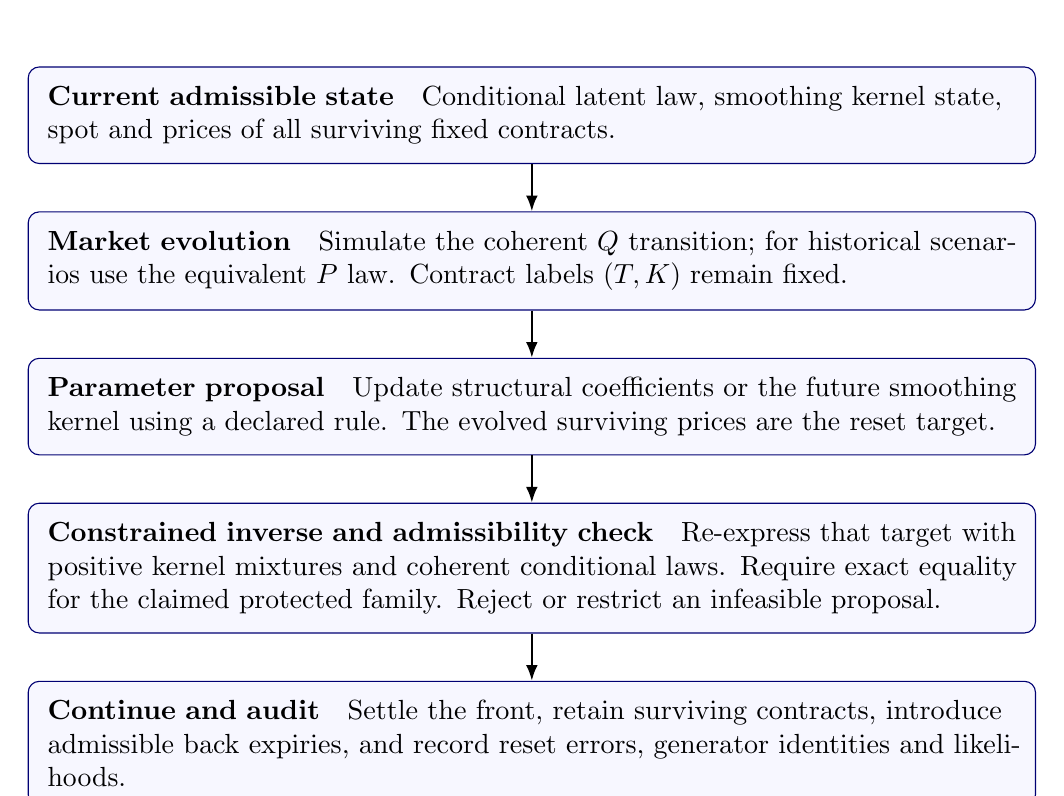
\begin{tikzpicture}[node distance=6mm,box/.style={draw=blue!45!black,rounded corners,fill=blue!3,text width=12.3cm,align=left,inner sep=7pt},arr/.style={-{Latex[length=2mm]},thick}]
\node[box] (a) {\textbf{Current admissible state}\quad Conditional latent law, smoothing kernel state, spot and prices of all surviving fixed contracts.};
\node[box,below=of a] (b) {\textbf{Market evolution}\quad Simulate the coherent $Q$ transition; for historical scenarios use the equivalent $P$ law. Contract labels $(T,K)$ remain fixed.};
\node[box,below=of b] (c) {\textbf{Parameter proposal}\quad Update structural coefficients or the future smoothing kernel using a declared rule. The evolved surviving prices are the reset target.};
\node[box,below=of c] (d) {\textbf{Constrained inverse and admissibility check}\quad Re-express that target with positive kernel mixtures and coherent conditional laws. Require exact equality for the claimed protected family. Reject or restrict an infeasible proposal.};
\node[box,below=of d] (e) {\textbf{Continue and audit}\quad Settle the front, retain surviving contracts, introduce admissible back expiries, and record reset errors, generator identities and likelihoods.};
\draw[arr] (a)--(b);\draw[arr] (b)--(c);\draw[arr] (c)--(d);\draw[arr] (d)--(e);
\end{tikzpicture}
\caption{Consistent recalibration in the SANOS/DYSANOS coordinates. The price move is produced by the stochastic transition; the subsequent coordinate reset preserves the evolved prices.}
\label{fig:crc}
\end{figure}

\subsection{A stitching theorem for price-preserving resets}
\begin{proposition}[Finite consistent recalibration]
\label{prop:stitch}
Consider finitely many ordered reset times before $T_*$. On each interval, choose an admissible conditional product model, or another common martingale model, for spot and a protected family of surviving contracts. Assume measurable conditional transition kernels, integrability sufficient for true martingality, and correct contractual settlement. At each reset, let the new model start from the old spot and the old values of every protected surviving contract, pathwise. Then the concatenated prices are martingales under the law obtained by concatenating these $Q$ kernels. If the protected family contains all strikes and relevant expiries, the full stated surface retains dynamic no-arbitrage.
\end{proposition}
\begin{proof}
For two times within an interval, the conditional martingale identity is part of the chosen model. At a reset, the price before and after coordinate replacement is equal. Applying conditional expectation across that reset therefore leaves the pre-reset value unchanged. Induction over the finite number of reset times proves the tower property across arbitrary intervals. Settlement identifies the final cashflow. The same law is used for the whole protected family.
\end{proof}
This is a sufficient stitching principle, not a theorem that the required inverse always exists. Preserving finitely many quotes preserves only that finite protected family at the reset. Full continuum preservation requires equality of the conditional call laws, equivalently their strike distributions at each surviving expiry, and can be much more restrictive. If a reset is intended to be an actual newly revealed market shock rather than a coordinate change, its price jump must instead satisfy the corresponding conditional martingale restriction; it cannot be declared price-preserving.

\subsection{An implementable order of estimation}
A constrained historical estimation problem can be written schematically as
\begin{equation}
 \min_{\vartheta,\lambda,z_{0:n}}
 \sum_{k,a}\mathcal E_{\rm quote}\!\left(H_a(t_k,z_k;\vartheta),c_{k,a}^{\rm obs}\right)
 -\sum_{k}\log p^{P,\vartheta,\lambda}_{\Delta t_k}(z_{k+1}\mid z_k)
 +\mathcal R(\vartheta,\lambda,z_{0:n}),
 \label{eq:joint-fit}
\end{equation}
subject to the exact structural constraints described below. The quote error can vanish inside bid--ask intervals. The transition density may be replaced by a justified likelihood approximation or another proper statistical score. $\mathcal R$ controls complexity, roughness and risk-premium size; it is not a replacement for martingale constraints.

The practical sequence is:
\begin{enumerate}[label=\textbf{\arabic*.},leftmargin=*]
\item \textbf{Fix the market and coordinates.} Declare the protected contracts, cash strikes, calendar expiries, observation times, tail treatment and settlement rule. Separate latent anchors from observed strikes. Decide whether the all-maturity chain model or the continuous model-expiry construction is used.
\item \textbf{Fit static states jointly with smoothing.} For proposed anchors and clock, solve the positive kernel calibration with mass, mean and latent convex-order constraints. With fixed kernels these are linear constraints. Retain bid--ask feasibility information and distinguish exact equality from approximation.
\item \textbf{Fit admissible risk-neutral transitions.} Choose martingale couplings, chain generators satisfying $Ax=0$, or Brownian revelation parameters. Require an actual conditional density tower. Derive the induced DLV drift rather than estimate it as a free parameter. If starting from arbitrary DLV loadings, verify existence, positivity and front closure separately.
\item \textbf{Fit physical risk premia.} Estimate $\lambda$ and, if relevant, positive jump-intensity tilts. Set the physical drift through \eqref{eq:girsanov} or \eqref{eq:jump-girsanov}. Check span, conditioning and likelihood integrability. Record $P$- and $Q$-dynamics in the same state coordinates.
\item \textbf{Refine the historical fit jointly.} Adjust latent states, the admissible transition family and nonidentified smoothing choices using \eqref{eq:joint-fit}. Repeated daily fitting with unconstrained parameter jumps is not a dynamic model. If the data cannot be explained within the current family, enlarge that family or report the misspecification.
\item \textbf{Specify the reset rule before simulation.} Simulate market evolution first; preserve its resulting prices during any parameter re-expression. Introduce new expiries through admissible extensions. If only a finite book is protected, state that restriction in the reported guarantee.
\item \textbf{Evaluate independently.} Test quote fit, forecast and hedging performance on held-out dates and regimes. Audit exact identities before using OCE or Monte Carlo mean tests.
\end{enumerate}
In observed data, today's surface is exogenous information to a filtering and estimation procedure. In a simulator, today's surface must be generated by its stochastic law. These roles should not be confused. A filter can update beliefs after an observation; a simulated price cannot be manually moved to a desired target and still inherit a martingale proof merely from static recalibration.

\subsection{What is fixed and what is recalibrated}
\begin{center}
\small
\begin{tabularx}{\textwidth}{@{}>{\raggedright\arraybackslash}p{.21\textwidth}>{\raggedright\arraybackslash}X>{\raggedright\arraybackslash}X@{}}
\toprule
Quantity & During a simulated interval & At a coordinate reset\\
\midrule
Surviving $(T,K)$ & Fixed contractual identity & Retained until settlement\\
Spot and call prices & Evolve under the selected $P$ or $Q$ law & Preserved for the protected family\\
Latent probabilities & Conditional-law evolution, not arbitrary fitting & May change if the same protected prices and a coherent continuation can be represented\\
DLV coordinates & Derived from the relevant latent or observed call book & Recomputed from that same book\\
Smoothing kernel & Additive Black clock, or an enlarged stochastic-volatility state with its full generator & Future kernel may change only with an admissible compensating recalibration\\
Risk-neutral coefficients & Prescribed admissible transition rule & May be updated within the admissible family\\
Physical risk premia & Adapted coefficients of an equivalent measure & May be re-estimated; likelihood and support conditions still apply\\
\bottomrule
\end{tabularx}
\end{center}
This is a programme for consistent estimation, not a guarantee of statistical accuracy. In particular, no-static-arbitrage is different from ``no statistical arbitrage''. Under $P$, economically meaningful risk premia and positive expected returns can remain.

\section{Reconciliation with the statistical DYSANOS Version 2.0 draft}
\label{sec:statistical-bridge}
The supplied \emph{DYSANOS}, Version~2.0 of 25 September 2026, by Buehler, Horv\'ath, Kratsios and Wiese \cite{DYSANOSv2}, is a statistical simulator built on SANOS. Its version number is separate from the working label ``DYSANOS II'' used for the present conditional-law research manuscript. The distinction is one of model specification and claims, not authorship. This section consolidates the two descriptions without attributing an unproved risk-neutral guarantee to the fitted statistical law.

\subsection{Two term structures, three meanings of time dependence}
Definition~3.1 of the statistical draft, reproduced in the supplied image, already has two term structures. Restoring a trading-date subscript $t$, its equation~(10) reads
\begin{align}
 \widetilde W_t^j&=\sum_{\ell=1}^j\sigma_t^\ell\sqrt{\Delta\widehat T^\ell},\notag\\
 W_t^j&=\eta_t^{\rm f}\sigma_t^1\sqrt{\Delta\widehat T^1}
       +\eta_t^{\rm term}\sum_{\ell=2}^j\sigma_t^\ell\sqrt{\Delta\widehat T^\ell}.
 \label{eq:dy2-clocks}
\end{align}
The first determines the relative strike support from front- and last-expiry normalised-moneyness candidates. The second supplies the Black smoothing total volatility. Thus the purposes differ even though the curves share the positive $\sigma^\ell$ coordinates. Two separately learned factors let front and later-expiry smoothing vary differently.

Here $W$ is a \emph{total standard deviation}; the corresponding argument of this paper's Black kernel is
\begin{equation}
 w_t(T)=[W_t(T-t)]^2.
 \label{eq:dy2-variance-map}
\end{equation}
The original SANOS production convention instead specifies a fraction $\mu$ of ATM \emph{total variance}, $w=\mu V_{\rm ATM}$. These conventions agree when $W=\sqrt\mu\,\sqrt{V_{\rm ATM}}$. If the two factors in \eqref{eq:dy2-clocks} both equal $\eta$, then $W=\eta\widetilde W$ and $w=\eta^2\widetilde W^2$; an amplitude multiplier is not the same numerical parameter as a variance multiplier. The reported preprocessing in \cite{DYSANOSv2}, footnote~4, uses $50\%$ of ATM total volatility, corresponding to $25\%$ of ATM variance. Its equation~(10) is written as a sum of total-volatility increments, not the usual square root of summed variance increments. It should be translated as printed rather than silently replaced by a different clock.

There are three distinct statements:
\begin{enumerate}
\item \emph{Across expiries at one date:} $W_t(\tau)$ is already nonconstant in maturity. No extension of SANOS is needed for this.
\item \emph{Across simulated dates:} the statistical latent state changes the fitted $\sigma_t^\ell$ and $\eta_t$ coordinates, so smoothing curves are already random along historical-style paths. Static admissibility can hold at every such date.
\item \emph{For one underlying smoothing process under $Q$:} the kernel must be its actual conditional-price function. Arbitrarily updating the fitted curve is not sufficient. A single Black kernel obeys Proposition~\ref{prop:black-rigidity}; a stochastic-volatility background uses Theorem~\ref{thm:sv-product} and generally a different pricing kernel.
\end{enumerate}

Any increasing absolutely continuous initial curve $W_0(T)$ with $W_0(0)=0$ can define a deterministic Black clock $V_Y(T)=W_0(T)^2$, with $\sigma_Y^2(T)=V_Y'(T)=2W_0(T)W_0'(T)$ almost everywhere. This includes the draft's monotone piecewise-linear interpolation of total volatility. Under that fixed law, however, the surviving contract's future variance is $V_Y(T)-V_Y(t)$; it is not an independently refitted $W_t(T-t)^2$. Linking that latter curve to the market state requires the full joint drift or price-preserving recalibration conditions.

In particular, tying the smoothing volatility to an ATM quantity depending on the $X$ state may destroy the independence required for the separated-kernel formula. Independent Brownian shocks alone do not imply independence of the complete subsystems. An orthogonal product can still be a martingale under appropriate integrability, but its prices must then be computed from the joint conditional law. Also, $\eta_{\min}>0$ in the draft is not a positive \emph{remaining variance floor}: $W_t(\tau)$ may still tend to zero as $\tau\downarrow0$. Proposition~\ref{prop:gb-floor} must not be used to reject that parametrisation.

\subsection{What the statistical draft already supplies}
The supplied draft already provides the smooth statically admissible SANOS decoder, positive DLV recursion, moving relative-grid geometry, and an affine map $u_t=b+B h_t$ with $h_t\in\R^{200}$. The two smoothing coordinates are part of that fitted map. It includes a stable weekly AR(1), Gaussian and heavy-tailed innovations, a scalar log-variance innovation factor, a conditional front-expiry spot copula, and evaluation of fixed cash contracts using remaining maturity and spot-relative strike. These are substantive implementation and empirical contributions.

Its reported experiment uses 891 SPX dates and approximately 3.57 million quotes. The daily-plus-weekly affine model places $80.9211\%$ inside bid--ask, compared with $72.8728\%$ for the weekly geometry. The improvement from explicit 1D--4D nodes is not a theorem about terminal settlement, but is meaningful evidence about short-end representation capacity. The draft also reports a full nonsingular 200-dimensional innovation covariance; the earlier 25-factor discussion must not be treated as the specification of this current checkpoint. These are reported findings of \cite{DYSANOSv2}, not independently reproduced experiments here.

Its no-replay log-variance factor controls the size of historical \emph{surface-state innovations}. It is not, by that fact alone, the risk-neutral return volatility of the multiplicative pricing factor $Y$. The path-distribution tests compare decoded scenarios statistically; they do not test the conditional martingale identities of every surviving option. The draft explicitly says this in its introduction on page~5 and in Section~4.8 on page~25. Its front-spot quantile construction supplies the current option-implied one-step marginal and a fitted spot--surface dependence, while deliberately not adding a physical spot drift. Matching that marginal does not also establish
\begin{equation}
 \E_Q[C_{t+\Delta}(T,K)\mid\F_t]=C_t(T,K)
 \quad\text{for every surviving fixed }(T,K).
 \label{eq:dy2-missing-tower}
\end{equation}
The simulator has a valid joint sampling rule, but the common pricing tower is an additional restriction on that rule.

The data claims must retain their stated qualifications: the shared decoder and baseline law are fitted using all dates; the 2025 evaluation is not an untouched forecast test of the whole model. Tail extensions improve the Gaussian baseline but still underproduce multiweek extremes. These findings motivate a richer generator; they cannot be relabelled as numerical validation of the present conditional-law construction.

\subsection{Overlap with SANOS, and the defensible additional contribution}
The central product observation is inherited. Original SANOS Theorem~3.1 already admits general positive background martingales, and Remark~3.2 already states the independent-product construction and names Heston as a possible background. Section~3.4 additionally discusses component-dependent kernels and a diffusion extension \cite{SANOS}. The statistical draft's Remark~2.7 likewise allows replacing the Black pricing function. Accordingly, neither deterministic maturity dependence, the product $XY$, nor the \emph{possibility} of a non-Black background should be presented as a new discovery of this manuscript.

The additional work relative to the supplied statistical draft is the explicit choice of coherent conditional laws through trading time; the fixed-contract generator and settlement calculations; the Wiese--Wissel and Carmona--Nadtochiy coordinate reconciliation; the exact-fit and rigidity propositions; and the constrained $P/Q$ calibration and numerical-audit programme. The general conditional-expectation argument is standard. Several auxiliary proofs are short consequences of known martingale, coupling, It\^o or moment-explosion results. ``Additional to the draft'' is therefore not a claim of established publication priority.

\begin{longtable}{@{}p{0.24\textwidth}p{0.32\textwidth}p{0.38\textwidth}@{}}
\caption{Scope of the consolidation. References to the statistical draft are to \cite{DYSANOSv2}; section references without that qualification refer to this manuscript.}\label{tab:dy2-scope}\\
\toprule Topic & Already established in the supplied lineage & Additional result and its importance\\\midrule\endfirsthead
\toprule Topic & Existing result & Additional result and its importance\\\midrule\endhead
Smoothness, static no-arbitrage and two curves & SANOS and statistical draft Sections~2--3. & A notation and clock dictionary; essential for consistency, not a new model principle.\\[3pt]
Independent product and general background & Original SANOS Theorem~3.1 and Remark~3.2; statistical draft Remark~2.7. & Conditional pricing, explicit generators and true-martingale assumptions. Useful operational detail; the core idea is inherited.\\[3pt]
Full fixed-contract dynamics & Statistical draft explicitly makes no dynamic pricing claim. & A coherent $Q$ construction with off-grid calls and settlement. Central theoretical addition relative to this draft, but it constructs its own dynamics.\\[3pt]
Finite and smooth drift restrictions & Wiese/Wissel and Carmona--Nadtochiy are predecessors. & Exact coordinate dictionary, jump corrections and diagnostics. Important for implementation and audit; not a newly discovered general drift principle.\\[3pt]
Front expiry & Daily nodes and a front-law spot copula are implemented. & Full conditional-law completion, continuous revelation examples and terminal obstruction proofs. Important for consistency through expiry; arbitrary fitted back-month dynamics remain unproved.\\[3pt]
Exact node matching and Bates & No corresponding results in the statistical draft. & Local positive-smoothing feasibility, finite-mixture obstruction, exact continuous mixing and independent controls. Useful to delimit what fitting and numerical tests can establish.\\[3pt]
Historical fit and computation & Extensive fitted model and empirical diagnostics in the statistical draft. & A constrained calibration programme and existence examples, not a completed equally accurate empirical simulator. Practical superiority remains untested.\\[3pt]
Risk premia and sample diagnostics & Statistical generation is specified; a joint equivalent pricing law is not established there. & Span/support conditions, price-preserving resets, OCE/ESS interpretation. Important methodology; existence and stable estimation for the actual fitted checkpoint remain open.\\
\bottomrule
\end{longtable}

\subsection{What is needed to connect the fitted simulator to the construction}
At zero carry, the cash price corresponding to the draft's normalised decoder is
\[
 H(t,s,h;T,K)=s\,c(h;T-t,K/s).
\]
The factor $s$, the remaining-time clock, and the changing relative strike all enter its generator. The statistical draft already specifies how to query fixed contracts; the new requirement is to constrain their \emph{evolution}, not merely relabel them. A compatible diffusion model would need
\begin{equation}
 (\partial_t+\mathcal L^Q)H=0,\qquad
 b^P-b^Q=\Sigma\lambda,
 \label{eq:dy2-compatible-drift}
\end{equation}
for the common state, together with terminal consistency and an admissible likelihood process. In a discrete simulator the corresponding requirements are the conditional tower and an equivalent change of transition law, not an assumed continuous-time formula. Full-rank latent innovation covariance does not guarantee that an arbitrary compressed decoder admits a drift satisfying every option equation: the Hessian contribution must be representable by the available state derivatives. Nor does a full-rank Gaussian weekly covariance identify the number of continuous Brownian factors without a specified embedding.

The theorem-backed route is therefore to retain the static fitting machinery while estimating a transition law inside a coherent conditional-pricing family, or to solve and validate \eqref{eq:dy2-compatible-drift} for the actual fitted decoder. Reusing its $200$ coordinates, two smoothing factors and observed spot copula unchanged is a stronger compatibility problem. Moving relative grids also need the cash-price-preservation constraints of Section~\ref{sec:regrid}; our fixed-latent-support examples do not prove arbitrary grid relocation harmless.

\subsection{Three source-level checks before numerical integration}
The following checks concern the printed draft, not a demonstrated defect in its code.
\begin{enumerate}
\item Its page~5 Black definition prints the same expression for both $d_+$ and $d_-$. For total standard deviation $W$, the intended quantities are $d_\pm=\log(S/K)/W\pm W/2$. The kernel in this manuscript uses that convention.
\item Its page~9 equation~(6) uses a product of adjacent strike gaps, whereas its following tridiagonal coefficients use their sum. For slope-difference masses $q_i$ and the usual irregular-grid generator, the coordinate identity is
\[
 \frac{c_i^j-c_i^{j-1}}{\Delta T_j}
   =\frac{\ell_i^j K_i^2}{h_i^++h_i^-}\,q_i^j,
 \qquad h_i^\pm=|K_{i\pm1}-K_i|.
\]
If the product-gap convention is intentional, its DLV must be rescaled by $h_i^+h_i^-/(h_i^++h_i^-)$ to represent this $\ell$. On moving grids that scaling has its own dynamics. The text and implementation must settle the convention before comparing drift coefficients.
\item A stable Gaussian weekly AR transition does not alone guarantee a valid fractional-time Gaussian diffusion. If $P$ is its invariant covariance and $A=e^{-\kappa}$, the proposed $Q_\Delta=P-e^{-\kappa\Delta}Pe^{-\kappa^\top\Delta}$ is positive semidefinite for every $\Delta\geq0$ exactly when
\begin{equation}
 D=\kappa P+P\kappa^\top\succeq0,
 \qquad Q_\Delta=\int_0^\Delta e^{-\kappa u}D e^{-\kappa^\top u}\dd u.
 \label{eq:dy2-embedding}
\end{equation}
Necessity follows by differentiating at zero; sufficiency follows from the integral. Dissipativity of $\kappa$ and a positive weekly $Q_1$ do not imply this for arbitrary fitted $P$. For example, $\kappa=\diag(1,10)$ and $P=\left(\begin{smallmatrix}1&0.9\\0.9&1\end{smallmatrix}\right)$ give a positive $Q_1$ but a negative eigenvalue of $Q_{0.01}$. The supplied checkpoint may pass the condition; it has not been inspected here. The exact OU update of the scalar log-variance factor likewise does not by itself specify the integrated covariance of a continuously varying-volatility surface-state diffusion.
\end{enumerate}
These checks can be resolved independently of the main distinction: the statistical simulator supplies fitted scenario dynamics, while the present construction supplies conditional-pricing identities for a specified coherent law. Demonstrating both properties in the \emph{same} fitted and efficiently simulated model remains the substantive joint objective.


\section{Verification: identities, numerical schemes and sampled markets}
\label{sec:testing}
\subsection{A hierarchy that separates causes of failure}
The construction provides an analytical statement. A discretisation and an estimated generator are additional objects. Sampling error can make a correct model look inconsistent, while a weak test can miss genuine bias. A defensible audit therefore proceeds in the following order.
\begin{enumerate}[label=\textbf{\arabic*.},leftmargin=*]
\item \textbf{Contract and law consistency.} Check fixed cash strikes and expiries, front settlement, tails, and the same underlying terminal law for spot and calls. Verify mass, mean, conditional-tower and price-preserving reset equalities.
\item \textbf{Deterministic drift identities.} Use one decoder, one generator, one clock and one jump convention for prices and all derivatives. Check \eqref{eq:ww}, \eqref{eq:decoder}, \eqref{eq:explicit-drift} or \eqref{eq:jump-drift} on all protected nodes and an independent dense off-grid set. A failure of an exact coordinate identity is not explained by coarse strike spacing.
\item \textbf{Boundary and numerical regularity.} Identify zero densities, near-singular inverse calibrations, nonsmooth active-set changes and maturity limits. Report excluded states. Confirm the claimed convergence under time-step refinement and independent derivative calculations.
\item \textbf{Conditional Monte Carlo moments.} Test the full protected book, including contracts near the tails and near expiry. Use independent path blocks and economically scaled confidence intervals. A large $p$-value does not prove equality, and an isolated small $p$-value among many tests does not by itself identify a model defect.
\item \textbf{Economic challenger tests.} Train hedging or OCE strategies independently, evaluate on held-out paths, and separate statistical risk premia from pathwise arbitrage. Check weight concentration and rare-event coverage before interpreting reweighting failures.
\end{enumerate}
The all-maturity chain example permits exact transition simulation and exact Black increments, so its martingale audit need not be contaminated by an Euler scheme. The Brownian revelation example permits direct evaluation of conditional probabilities. These are useful benchmark implementations against which a more flexible learned simulator can be tested.

\subsection{OCE as a diagnostic and a measure selector}
Let $\Delta C_{k+1}$ denote gains of the \emph{same} fixed contracts, including settlement when an expiry is crossed. For a predictable strategy $a$, write $G(a)=\sum_ka_k\cdot\Delta C_{k+1}$. Let $u$ be increasing and concave, with $u(0)=0$ and $u'(0)=1$. The optimised certainty equivalent problem is
\begin{equation}
 V_P=\sup_{a,c}\{\E_P[u(c+G(a))]-c\}.
 \label{eq:oce}
\end{equation}
Under the constructed $Q$, for strategies with integrable zero-mean gains, concavity gives $u(x)\leq x$, hence $V_Q\leq0$. The zero strategy and $c=0$ attain zero. Therefore the ideal population benchmark is $V_Q=0$. Under $P$, $V_P$ can be positive because of ordinary risk premia; this is not by itself a classical arbitrage.

\begin{proposition}[The interior OCE first-order condition]
\label{prop:oce}
Suppose a finite optimum $(a^*,c^*)$ exists, $u'>0$, differentiation under expectation is justified, and the strategy space allows both signs of all bounded predictable perturbations in the protected assets. Then
\begin{equation}
 D^*=u'(c^*+G(a^*))>0,\qquad \E_P[D^*]=1,
 \label{eq:oce-density}
\end{equation}
and $dQ^*=D^*dP$ makes the protected discrete-time gains conditionally mean zero.
\end{proposition}
\begin{proof}
Differentiating in $c$ yields $\E_P[D^*]=1$. A perturbation that holds the $j$th asset over one period on an arbitrary event $A\in\F_{t_k}$ yields
$\E_P[D^*\ind_A\Delta C^j_{k+1}]=0$. This is equivalent to the conditional martingale increment identity under $Q^*$, since the conditional density is strictly positive. Positivity and normalisation give an equivalent probability measure.
\end{proof}
This is the frictionless population mechanism behind OCE-based drift removal \cite{OCE}. A neural strategy class tests only its available perturbations. Transaction costs or trading constraints change the conclusion to inequalities or a near-martingale statement. Existence of a finite optimum and the required moments are substantive assumptions; a finite training sample does not establish them. In an incomplete market the selected $Q^*$ also need not equal the product construction's chosen $Q$.

For exponential utility, optimising over the cash shift gives $-\gamma^{-1}\log\E[e^{-\gamma G}]$. In the special one-period Gaussian case, $G=aR$, with mean $\mu$ and variance $v>0$, maximisation over $a$ gives $\mu^2/(2\gamma v)$. OCE is therefore not generally ``mean divided by variance''. Exponential integrability can fail for unbounded short-option losses; the utility and strategy class must be selected accordingly.

\subsection{Why span and ESS are separate diagnostics}
The span residual \eqref{eq:span-residual} asks whether an equivalent drift change is possible for the specified coefficients. Effective sample size asks whether a \emph{particular finite sample} can estimate expectations under a chosen density ratio:
\begin{equation}
 \ess=\frac{(\sum_{n=1}^ND_n)^2}{\sum_{n=1}^ND_n^2}.
 \label{eq:ess}
\end{equation}
For constant Brownian $\lambda$ and horizon $T$, $\E_P[D^2]=e^{\|\lambda\|^2T}$, so the large-sample ESS fraction is $e^{-\|\lambda\|^2T}$. An equivalent measure may exist while the effective sample is tiny. Conversely, no increase in sample size repairs a structural nonzero span residual for an incompatible prescribed diffusion drift.

For an independent one-step sample, strictly positive weights satisfying all empirical mean-zero constraints exist exactly when zero lies in the relative interior of the convex hull of the observed return vectors. A missing rare payoff event can make this empirical feasibility fail even when the population model is arbitrage-free. That failure concerns the finite empirical distribution. It is not a proof that the analytical law permits arbitrage. Dynamic feasibility must use the appropriate information and conditional branches; a path cloud with a unique observed successor at every state can create artificial predictability.

When the likelihood ratio is known from the fitted model, a useful out-of-sample family of checks is
\begin{equation}
 \E_P\left[D_{T_*}\,f(Z_{t_k})\Delta C^a_{k+1}\right]=0
 \label{eq:weighted-moments}
\end{equation}
for selected conditioning features $f$ and every protected asset $a$. Weight concentration, tail-event counts, simultaneous uncertainty and solver accuracy should accompany the residuals. These checks complement the structural proof; they do not replace it.

\section{Discussion and research implications}
The central conclusion is constructive. A finite density market and a smooth surface need not be competing descriptions. A coherent latent martingale, an independent smoothing martingale and conditional pricing give one common market. The Wiese--Wissel condition is its exact finite-grid coordinate restriction; the continuous covariance drift is the corresponding smooth identity, with the correct clock, closure and jump terms.

Section~\ref{sec:bates} sharpens the role of an affine oracle such as generalised Bates: its nondegenerate marginal cannot be represented by a finite Black mixture, whereas a continuous anchor--variance mixture is exact. These representation results do not obstruct a different coherent finite SANOS market. An oracle is valuable for testing decoders, numerical derivatives and drift calculations against a known law. Exact representation of its full surface is not required to build an arbitrage-free SANOS-type market. Nor does a good static approximation to that oracle inherit its dynamics. The appropriate test is whether the \emph{fitted decoder under its declared generator} has zero drift and correct settlement. The Black product model supplies an independent constructive benchmark for that test.

Common-node matching has a precise scope. Positive smoothing with frozen atomic weights changes prices. Joint calibration can restore protected quotes, and a strict finite book admits a nonzero smoothing interval under Theorem~\ref{thm:local-fit}. Thereafter a coherent law determines both its grid and off-grid evolution. Preserving an externally specified full DLV trajectory, or changing a finite-mixture clock while preserving a whole continuum of quotes, remains a stronger inverse problem and may be infeasible.

The resulting historical calibration problem is constrained but not circular. Admissible $Q$ transitions determine the allowed drift geometry; risk premia choose compatible $P$ dynamics; cross-sectional observations and transition statistics select among the remaining freedoms. Reducing tradables, reducing state dimension and reducing Brownian drivers are distinct choices. CRC-inspired resets are useful only when their correction preserves the family for which the no-arbitrage claim is made.

The fitted statistical model is not automatically an instance of these existence examples. Its compressed decoder, moving grid, historical covariance, smoothing updates and spot copula still need a common admissible pricing law; the product theorem alone does not provide that compatibility. The main open implementation questions include efficient estimation of a sufficiently rich latent transition family, robust inverse calibration at large smoothing levels, long-horizon support management, and stable simulation close to settlement. These do not negate the proved existence examples. They determine whether the guaranteed model family is rich and economical enough for useful deep-hedging experiments.

\appendix
\section{A compact specification for a reproducible implementation}
\label{app:implementation}
An implementation should export the following objects separately rather than store only surface snapshots:
\begin{enumerate}
\item The latent anchor array $x$, protected cash strikes $K$, calendar expiries $T$, and the time grid. Record the distinct meaning of latent weights and observed butterflies.
\item The additive Black variance clock, latent initial probabilities and martingale transition matrices or generator. For the Brownian construction, store the transition thresholds in \eqref{eq:revelation}.
\item The kernel calibration equations, their exact or bid--ask targets, positivity and convex-order margins, and inverse conditioning diagnostics.
\item The decoder, its analytic or validated automatic derivatives, and both $Q$ and $P$ generators in one convention. Store the full measure-change likelihood, including reset or jump terms where applicable.
\item Every original surviving contract's chronological prices and settlement. A floating display grid can be exported as an additional view, never as a replacement for the fixed-contract audit.
\item The full set of structural residuals, conditional sample moments, independent OCE evaluation, ESS and rare-event coverage. Report all exclusions and the reasons for them.
\end{enumerate}

For the finite-chain benchmark, simulate the chain using its exact time-homogeneous transition matrix or a valid nonhomogeneous-chain algorithm, and simulate Black increments exactly. Reprice by \eqref{eq:chain-price}. For the revelation benchmark, simulate Brownian increments and evaluate \eqref{eq:revelation}--\eqref{eq:tower-revelation} directly. These benchmarks distinguish a model error from an error introduced by a generic SDE discretisation.

A minimal verification example uses \eqref{eq:three-state} with $r>0$, $\sigma_Y>0$, several fixed expiries, and a dense set of cash strikes. The exact generator residual is zero by \eqref{eq:chain-pde}; this is an analytic identity, not a reported numerical outcome. The finite butterfly and calendar ratios must reproduce the jump version of the Wiese--Wissel condition when evaluated from this same decoder. A diffusion-only residual would be the wrong diagnostic for this example.

\section{Attribution and the status of the combined results}
This manuscript consolidates the supplied density-DLV, exact Black-product, Carmona--Nadtochiy/CRC, and extended calibration notes, together with the two Bates/SANOS analyses dated 23 and 24 September 2026 \cite{BatesCompatibility,FiniteSANOS}. The presentation supplies motivation and background only. The finite-density derivation is credited to Wiese's discussion note \cite{WieseNote}; the reconciliation identifies its established Wissel predecessor. The static product interpretation is already part of the SANOS lineage and is not claimed here as a newly discovered static parametrisation.

The detailed developments collected here are the conditional-law formulation, settlement and between-strike generator calculations, finite-chain and Brownian-revelation examples, and the local positive-smoothing exact-fit argument with its limitations. The independent-product principle, general background martingales (including Heston), and maturity-dependent smoothing are already in SANOS. The single-Black rigidity calculation is a direct consistency calculation, related to the flat-smile result in \cite{SSVI}. Additional detail relative to the supplied statistical draft is not, by itself, an established claim of mathematical priority; Table~\ref{tab:dy2-scope} states the comparison precisely. Section~\ref{sec:bates} incorporates the additional proofs and examples from those analyses; Table~\ref{tab:bates-audit} attributes their numerical observations without claiming a fresh run or inspection of the underlying code. The historical calibration procedure is a research methodology constrained by those results; its statistical effectiveness still requires experiments. The exact numbered reference to Wissel's 2007 equation follows the supplied reconciliation note; the full algebraic relation is restated in \eqref{eq:wissel} so the proof does not rely on an inaccessible equation label. A submission version should archive the exact 2007 source alongside that reference.
\appendix
\section{Prompt for CRC}
TASK: Implement and evaluate a CRC-inspired, dynamically consistent
extension of the existing DYSANOS statistical simulator.

OBJECTIVE

The existing DYSANOS model jointly fits DLV coordinates, grid geometry,
smoothing parameters and statistical state dynamics. Its decoder ensures
static arbitrage-free snapshots. Its reported “consistent P-simulation”
does not establish a common pricing measure for surviving contracts.

Construct and test an admissible modification of this model. The existing
AR(1) law is an empirical baseline and fitting target, not an immutable
constraint.

The research question is:

Can we retain useful quote fit and historical transition behaviour while
imposing coherent Q-dynamics, compatible P-dynamics and price-preserving
recalibration?

Do not substitute a test of whether the original unconstrained AR(1)
already happens to satisfy those conditions.

CONTEXT AND ATTRIBUTION

Use the supplied DYSANOS draft and the accompanying smooth-DYSANOS
construction as specifications to examine critically.

The independent-product idea, general background martingales and
maturity-dependent smoothing already occur in SANOS. Do not claim these
as new.

The proposed additional work is the integration of conditional pricing,
Wiese/Wissel drift compatibility, admissible historical dynamics and
consistent recalibration into a fitted simulator.

Treat the accompanying manuscript as a research specification requiring
verification, not as authority that an arbitrary fitted decoder admits
the required dynamics.

1. AUDIT THE EXISTING IMPLEMENTATION

Identify the exact implementation and checkpoint used.

Document:
- the latent state and decoder;
- the mapping to DLV coordinates and density probabilities;
- the two term structures: grid geometry and smoothing;
- whether smoothing parameters scale variance or standard deviation;
- the statistical transition law and innovation covariance;
- the front-expiry spot law and spot–surface dependence;
- moving-grid, maturity-roll and settlement conventions;
- any actual pricing-drift or price-preserving-reset constraints.

Identify what is jointly estimated. Joint estimation alone must not be
reported as consistent recalibration.

Preserve the existing simulator as a reproducible baseline.

2. DEFINE THE MARKET AND THE PRICING IDENTITIES

Specify the numeraire, carry convention, filtration, traded contracts,
joint spot–surface state and expiry treatment.

At zero carry, if c is the normalized decoder, evaluate a fixed cash
contract through

  H(t,s,h;T,K) = s c(h; T-t, K/s).

Keep T and K fixed when following a surviving contract.

For a diffusion construction, impose

  $(partial_t + L_Q) H(t,z;T,K) = 0.$

Include all relevant state derivatives, covariance terms, the moving
moneyness, maturity clock, grid geometry and smoothing coordinates.
Include jump/reset terms where applicable.

For the actual discrete-time simulator, impose and test

  E_Q[H(t+Delta,Z_next;T,K) | Z_current]
      = H(t,Z_current;T,K),

with the correct settlement payoff if expiry is crossed.

A continuous-time drift formula does not certify an arbitrary finite
weekly step.

State whether the claimed guarantee covers:
(a) only a declared finite protected book; or
(b) the entire smooth surface through a common conditional-pricing law.

Do not infer (b) from finitely many numerical tests of (a).

3. ESTABLISH AN IMPLEMENTABLE ADMISSIBLE Q FAMILY

First determine whether the existing decoder admits the required
Q-dynamics for a useful volatility specification.

Derive the drift feasibility equations. Report their rank, conditioning
and residual, including off-grid restrictions.

If the exact compressed decoder is too restrictive, investigate clearly
identified modifications, for example:
- additional state coordinates;
- modified volatility loadings;
- density or transition-law coordinates;
- a coherent product-kernel representation.

Do not silently change the model and present it as the original model.

For an independent product construction:
- construct a coherent latent martingale X, including settlement;
- use a positive true martingale Y independent of the complete X system;
- price all calls by the same joint conditional expectation.

If Y has stochastic volatility, use its actual conditional pricing
kernel. Do not insert current random volatility into an otherwise
unchanged Black formula.

Verify true martingality for the selected Y specification. Distinguish
the Black-mixture implementation from any generalized-kernel extension,
and report the computational difference.

A certified structural benchmark may be implemented first. It must be
labelled a benchmark until it has been fitted and compared with the
empirical baseline.

4. FIT HISTORICAL DYNAMICS WITHIN THE ADMISSIBLE FAMILY

Use the existing AR(1) model to identify desirable empirical behaviour:
conditional means, covariance, persistence, cross-expiry dependence,
spot–surface dependence and tails.

For a diffusion parametrisation, fit P through

  b_P = b_Q + Sigma lambda,

using the same diffusion coefficient under equivalent measures.
Verify the likelihood process, not only the instantaneous span equation.

It is permissible to re-estimate Sigma and the representation jointly,
provided the Q restrictions are maintained.

For a discrete-time implementation, construct compatible P and Q
transition kernels with the required common support and valid positive
density ratios. A valid positive tilt of an admissible Q kernel is one
possible construction.

Do not force exact AR(1) form if it is incompatible. Instead report
precisely which properties are relaxed and why.

Fit against historical observations as well as comparing with the AR(1)
baseline. Matching an estimated baseline is not a substitute for
validation on data.

5. IMPLEMENT THE CONSISTENT RECALIBRATION SEQUENCE

Use the following order:

A. Initial calibration:
Jointly fit an admissible initial state and structural parameters to
the observed option book. Check static constraints and representability.

B. Market evolution:
Evolve the joint spot–surface model under its specified Q law, or under
its compatible P law for historical scenarios.

C. Update target:
Compute the evolved prices of the same surviving contracts. These
prices are the target that a pure parameter reset must preserve.

D. Structural parameter proposal:
Propose updated parameters using the estimation/filtering procedure.

E. Constrained inverse:
Find a representation under the proposed parameters that reproduces
the target prices exactly, subject to positivity, mean, calendar and
other model admissibility constraints.

F. Feasibility decision:
Accept only an admissible reset. If infeasible, reject it or make a
documented model adjustment and solve again. Report all such events.

G. Continue:
Carry forward the required conditional state, settle expired contracts
and introduce new expiries through an admissible extension.

Distinguish:
- stochastic market evolution;
- a price-preserving representation change;
- conditioning on newly observed data.

A newly observed market surface is not required to equal yesterday's
forecast. However, an arbitrary refit to that observation is not thereby
a price-preserving reset or a proof of dynamic consistency.

Verify that the new continuation model is coherent after each reset,
not merely that its prices agree at the reset instant.

If only a finite book is preserved, report off-grid reset price changes
and restrict the guarantee accordingly.

6. VALIDATE IN THE FOLLOWING ORDER

A. Structural checks:
Mass, positivity, conditional mean, static constraints, conditional
pricing identities, front settlement and recalibration feasibility.

B. Deterministic numerical checks:
Generator residuals and reset errors using one identical decoder and
consistent derivatives. Test all protected nodes, not a small subset.
Use an independent off-grid audit set and convergence checks.

C. Conditional Monte Carlo:
Test surviving fixed contracts conditional on representative starting
states, including tails and near-expiry states. Separate discretisation
bias, kernel approximation error and sampling error.

D. Historical performance:
Use chronological training and validation splits. Report quote fit,
transition likelihood or another justified proper score, covariance,
autocorrelation, tails, spot–surface dependence and simulation cost.
Retain the original all-history fit only as a labelled reconstruction
benchmark, not an out-of-sample result.

E. Economic diagnostics:
Use OCE or hedging tests as additional diagnostics, not substitutes for
the pricing identities. Report ESS only with the exact density ratio,
direction of reweighting and sample law specified.

7. REQUIRED REPORT AND ARTIFACTS

Produce a self-contained LaTeX report and compiled PDF containing:

- the implemented model and exact scope of its guarantee;
- a table of unchanged versus modified baseline components;
- the mathematical Q restrictions and P/Q compatibility conditions;
- a step-by-step recalibration diagram;
- chronological parameter and price examples before evolution,
  after evolution, and before/after each reset;
- baseline-versus-constrained quote-fit and dynamics comparisons;
- surface snapshots and off-grid residual plots;
- feasibility failures, conditioning and computational costs;
- a separation of proved identities, numerical evidence and open claims.

Export:
- configurations, seeds and checkpoint identifiers;
- chronological state and parameter arrays;
- protected contract identifiers;
- pre-/post-reset prices and residuals;
- reproducible commands and focused regression tests.

SUCCESS CRITERION

A successful outcome exhibits one clearly specified modified model
with defensible dynamic pricing consistency and quantified empirical
performance relative to the original AR(1) baseline.

It need not preserve the original AR(1) law exactly.

If that outcome cannot be achieved within the investigated family,
identify the specific mathematical or numerical obstruction and the
smallest justified modification to investigate next. Do not turn failure
of one parametrisation or numerical search into a universal
impossibility claim.

\begingroup\small
\begin{thebibliography}{99}
\bibitem{Wiese2019}
M.~Wiese, L.~Bai, B.~Wood and H.~Buehler.
\emph{Deep Hedging: Learning to Simulate Equity Option Markets}.
2019. \href{https://arxiv.org/abs/1911.01700}{arXiv:1911.01700}.

\bibitem{DeepHedging}
H.~Buehler, L.~Gonon, J.~Teichmann and B.~Wood.
Deep hedging. \emph{Quantitative Finance} 19(8), 1271--1291, 2019.
\href{https://arxiv.org/abs/1802.03042}{arXiv:1802.03042}.

\bibitem{Expensive}
H.~Buehler. Expensive martingales.
\emph{Quantitative Finance} 6(3), 207--218, 2006.

\bibitem{SANOS}
H.~Buehler, B.~Horv\'ath, A.~Kratsios, Y.~Limmer and R.~Saqur.
\emph{SANOS---Smooth Strictly Arbitrage-Free Non-Parametric Option Surfaces}.
2026. \href{https://arxiv.org/abs/2601.11209}{arXiv:2601.11209}.

\bibitem{DYSANOS}
H.~Buehler, B.~Horv\'ath and A.~Kratsios.
\emph{DYSANOS: Generative Dynamic Smooth Arbitrage-free Non-parametric Option Surfaces}.
2026. \href{https://arxiv.org/abs/2608.12587}{arXiv:2608.12587}.

\bibitem{Wissel2007}
J.~Wissel. \emph{Arbitrage-free market models for option prices}.
NCCR FINRISK / University of Zurich, Working Paper 428, 2007.
Finite-option preprint; distinguished here from the 2008 multi-strike article.

\bibitem{WisselThesis}
J.~S.~Wissel. \emph{Arbitrage-free Market Models for Liquid Options}.
Doctoral thesis, ETH Zurich, No.~17538, 2008.
\href{https://doi.org/10.3929/ethz-a-005559619}{doi:10.3929/ethz-a-005559619}.

\bibitem{SWMulti}
M.~Schweizer and J.~Wissel.
Arbitrage-free market models for option prices: the multi-strike case.
\emph{Finance and Stochastics} 12, 469--505, 2008.
\href{https://doi.org/10.1007/s00780-008-0068-6}{doi:10.1007/s00780-008-0068-6}.

\bibitem{SWTerm}
M.~Schweizer and J.~Wissel.
Term structures of implied volatilities: absence of arbitrage and existence results.
\emph{Mathematical Finance} 18(1), 77--114, 2008.
\href{https://doi.org/10.1111/j.1467-9965.2007.00323.x}{doi:10.1111/j.1467-9965.2007.00323.x}.

\bibitem{WieseNote}
M.~Wiese. \emph{A drift restriction for discrete local volatility: the argument in five steps}.
Discussion note, 24 August 2026. Unpublished research material, as identified in the supplied density-coordinate reconciliation.

\bibitem{CN2009}
R.~Carmona and S.~Nadtochiy. Local volatility dynamic models.
\emph{Finance and Stochastics} 13, 1--48, 2009.
\href{https://doi.org/10.1007/s00780-008-0078-4}{doi:10.1007/s00780-008-0078-4}.
Author preprint, 28 May 2007:
\href{https://carmona.scholar.princeton.edu/document/246}{Princeton author copy}.

\bibitem{CN2008}
R.~Carmona and S.~Nadtochiy.
An infinite dimensional stochastic analysis approach to local volatility dynamic models.
\emph{Communications on Stochastic Analysis} 2(1), 109--123, 2008.
\href{https://repository.lsu.edu/cosa/vol2/iss1/8/}{Author article}.

\bibitem{CN2012}
R.~Carmona and S.~Nadtochiy. Tangent L\'evy market models.
\emph{Finance and Stochastics} 16, 63--104, 2012.
\href{https://doi.org/10.1007/s00780-011-0158-8}{doi:10.1007/s00780-011-0158-8}.

\bibitem{KK2015}
J.~Kallsen and P.~Kr\"uhner. On a Heath--Jarrow--Morton approach for stock options.
\emph{Finance and Stochastics} 19, 583--615, 2015.
\href{https://doi.org/10.1007/s00780-015-0263-1}{doi:10.1007/s00780-015-0263-1}.

\bibitem{CRC}
M.~Gambara and J.~Teichmann.
\emph{Consistent Recalibration Models and Deep Calibration}.
2020, revised 2021. \href{https://arxiv.org/abs/2006.09455}{arXiv:2006.09455}.

\bibitem{ContFonseca}
R.~Cont and J.~da Fonseca. Dynamics of implied volatility surfaces.
\emph{Quantitative Finance} 2(1), 45--60, 2002.
\href{https://doi.org/10.1088/1469-7688/2/1/304}{doi:10.1088/1469-7688/2/1/304}.

\bibitem{CFD}
R.~Cont, J.~da Fonseca and V.~Durrleman.
Stochastic models of implied volatility surfaces.
\emph{Economic Notes} 31(2), 361--377, 2002.

\bibitem{ContVuletic}
R.~Cont and M.~Vuleti\'c. Simulation of arbitrage-free implied volatility surfaces.
\emph{Applied Mathematical Finance} 30(2), 94--121, 2023.
\href{https://doi.org/10.1080/1350486X.2023.2277960}{doi:10.1080/1350486X.2023.2277960}.

\bibitem{VolGAN}
M.~Vuleti\'c and R.~Cont. VolGAN: a generative model for arbitrage-free implied volatility surfaces.
\emph{Applied Mathematical Finance} 31(4), 203--238, 2024 issue; published online 2025.
\href{https://doi.org/10.1080/1350486X.2025.2471317}{doi:10.1080/1350486X.2025.2471317}.

\bibitem{CRW}
S.~N.~Cohen, C.~Reisinger and S.~Wang. Arbitrage-free neural-SDE market models.
\emph{Applied Mathematical Finance} 30(1), 1--46, 2023.
\href{https://arxiv.org/abs/2105.11053}{arXiv:2105.11053};
\href{https://doi.org/10.1080/1350486X.2023.2257217}{doi:10.1080/1350486X.2023.2257217}.

\bibitem{Dupire}
B.~Dupire. Pricing with a smile. \emph{Risk} 7(1), 18--20, 1994.

\bibitem{DLV}
H.~Buehler and E.~Ryskin. \emph{Discrete local volatility for large time steps}.
2015. \href{https://ssrn.com/abstract=2642630}{SSRN 2642630}.

\bibitem{AH}
J.~Andreasen and B.~Huge. Volatility interpolation. \emph{Risk}, March 2011, 86--89.

\bibitem{Strassen}
V.~Strassen. The existence of probability measures with given marginals.
\emph{Annals of Mathematical Statistics} 36(2), 423--439, 1965.
\href{https://doi.org/10.1214/aoms/1177700153}{doi:10.1214/aoms/1177700153}.

\bibitem{Kellerer}
H.~G.~Kellerer. Markov-Komposition und eine Anwendung auf Martingale.
\emph{Mathematische Annalen} 198, 99--122, 1972.

\bibitem{HullWhite1987}
J.~Hull and A.~White. The pricing of options on assets with stochastic volatilities.
\emph{Journal of Finance} 42(2), 281--300, 1987.
\href{https://doi.org/10.1111/j.1540-6261.1987.tb02568.x}{doi:10.1111/j.1540-6261.1987.tb02568.x}.

\bibitem{OCE}
H.~Buehler, P.~Murray, M.~S.~Pakkanen and B.~Wood.
\emph{Deep Hedging: Learning to Remove the Drift under Trading Frictions with Minimal Equivalent Near-Martingale Measures}.
2021, revised 2022. \href{https://arxiv.org/abs/2111.07844}{arXiv:2111.07844}.

\bibitem{BatesCompatibility}
Supplied research analysis. \emph{Exact Bates--DLV--SANOS compatibility: what exists, what does not, and how to test it}. 23 September 2026. Analysis of the supplied Task~7 report; unpublished working note.

\bibitem{FiniteSANOS}
Supplied research analysis. \emph{Finite SANOS dynamics without a Bates oracle: existence, drift compatibility and precise rigidity results}. 24 September 2026. Unpublished working note.

\bibitem{MomentExplosion}
M.~Keller-Ressel. \emph{Moment Explosions and Long-Term Behavior of Affine Stochastic Volatility Models}. Mathematics and Financial Economics 4, 73--98 (2011). Corollary~2.7, Theorem~4.1 and the Heston example in Section~6.1 of the preprint. \url{https://arxiv.org/abs/0802.1823}.

\bibitem{Jourdain2004}
B.~Jourdain. \emph{Loss of martingality in asset price models with lognormal stochastic volatility}. Preprint CERMICS 2004-267, 7 July 2004. Theorem~1 and Remark~2 distinguish lognormal volatility from square-root variance. \href{https://cermics.enpc.fr/cermics-rapports-recherche/2004/CERMICS-2004/CERMICS-2004-267.pdf}{Author preprint}.

\bibitem{InformationPricing}
D.~C.~Brody, L.~P.~Hughston and A.~Macrina. \emph{Information-Based Asset Pricing}. arXiv:0704.1976. \url{https://arxiv.org/abs/0704.1976}.

\bibitem{SSVI}
M.~El Amrani, A.~Jacquier and C.~Martini. \emph{Dynamics of symmetric SSVI smiles and implied volatility bubbles}. arXiv:1909.10272v3 (2021), Theorem~3.5, Proposition~3.6 and Section~3.3. \url{https://arxiv.org/abs/1909.10272}.


\bibitem{DYSANOSv2}
H.~Buehler, B.~Horv\'ath, A.~Kratsios and M.~Wiese.
\emph{DYSANOS: Generative Dynamic Smooth Arbitrage-free Non-parametric Option Surfaces}.
Supplied working draft, Version~2.0, 25 September 2026, 30 pages (\texttt{dy2.pdf}). Definition~3.1 and equations~(8)--(13); Sections~4.5 and~4.8. Distinct from the earlier three-author version cited above.

\end{thebibliography}
\endgroup
\end{document}
